% This template has been tested with LLNCS DOCUMENT CLASS -- version 2.20 (10-Mar-2018)

% !TeX spellcheck = en-US
% !TeX encoding = utf8
% !TeX program = pdflatex
% !BIB program = bibtex
% -*- coding:utf-8 mod:LaTeX -*-

% "a4paper" enables:
%  - easy print out on DIN A4 paper size
%
% One can configure a4 vs. letter in the LaTeX installation. So it is configuration dependend, what the paper size will be.
% This option  present, because the current word template offered by Springer is DIN A4.
% We accept that DIN A4 cause WTFs at persons not used to A4 in USA.

% "runningheads" enables:
%  - page number on page 2 onwards
%  - title/authors on even/odd pages
% This is good for other readers to enable proper archiving among other papers and pointing to
% content. Even if the title page states the title, when printed and stored in a folder, when
% blindly opening the folder, one could hit not the title page, but an arbitrary page. Therefore,
% it is good to have title printed on the pages, too.
%
% It is enabled by default as the springer template as of 2018/03/10 uses this as default

% German documents: pass ngerman as class option
% \documentclass[ngerman,runningheads,a4paper]{llncs}[2018/03/10]
% English documents: pass english as class option
\documentclass[english,runningheads,a4paper]{llncs}[2018/03/10]

%% If you need packages for other papers,
%% START COPYING HERE

% Set English as language and allow to write hyphenated"=words
%
% In case you write German, switch the parameters, so that the command becomes
%\usepackage[english,main=ngerman]{babel}
%
% Even though `american`, `english` and `USenglish` are synonyms for babel package (according to https://tex.stackexchange.com/questions/12775/babel-english-american-usenglish), the llncs document class is prepared to avoid the overriding of certain names (such as "Abstract." -> "Abstract" or "Fig." -> "Figure") when using `english`, but not when using the other 2.
% english has to go last to set it as default language
\usepackage[ngerman,main=english]{babel}
%
% Hint by http://tex.stackexchange.com/a/321066/9075 -> enable "= as dashes
\addto\extrasenglish{\languageshorthands{ngerman}\useshorthands{"}}
%
\usepackage{graphicx}
% Fix by https://tex.stackexchange.com/a/441701/9075
\usepackage{regexpatch}
\makeatletter
\edef\switcht@albion{%
  \relax\unexpanded\expandafter{\switcht@albion}%
}
\xpatchcmd*{\switcht@albion}{ \def}{\def}{}{}
\xpatchcmd{\switcht@albion}{\relax}{}{}{}
\edef\switcht@deutsch{%
  \relax\unexpanded\expandafter{\switcht@deutsch}%
}
\xpatchcmd*{\switcht@deutsch}{ \def}{\def}{}{}
\xpatchcmd{\switcht@deutsch}{\relax}{}{}{}
\edef\switcht@francais{%
  \relax\unexpanded\expandafter{\switcht@francais}%
}
\xpatchcmd*{\switcht@francais}{ \def}{\def}{}{}
\xpatchcmd{\switcht@francais}{\relax}{}{}{}
\makeatother

\usepackage{ifluatex}
\ifluatex
  \usepackage{fontspec}
  \usepackage[english]{selnolig}
\fi

\iftrue % use default-font
  \ifluatex
    % use the better (sharper, ...) Latin Modern variant of Computer Modern
    \setmainfont{Latin Modern Roman}
    \setsansfont{Latin Modern Sans}
    \setmonofont{Latin Modern Mono} % "variable=false"
    %\setmonofont{Latin Modern Mono Prop} % "variable=true"
  \else
    % better font, similar to the default springer font
    % cfr-lm is preferred over lmodern. Reasoning at http://tex.stackexchange.com/a/247543/9075
    \usepackage[%
      rm={oldstyle=false,proportional=true},%
      sf={oldstyle=false,proportional=true},%
      tt={oldstyle=false,proportional=true,variable=false},%
      qt=false%
    ]{cfr-lm}
  \fi
\else
  % In case more space is needed, it is accepted to use Times New Roman
  \ifluatex
    \setmainfont{TeX Gyre Termes}
    \setsansfont[Scale=.9]{TeX Gyre Heros}
    % newtxtt looks good with times, but no equivalent for lualatex found,
    % therefore tried to replace with inconsolata.
    % However, inconsolata does not look good in the context of LNCS ...
    %\setmonofont[StylisticSet={1,3},Scale=.9]{inconsolata}
    % ... thus, we use the good old Latin Modern Mono font for source code.
    \setmonofont{Latin Modern Mono} % "variable=false"
    %\setmonofont{Latin Modern Mono Prop} % "variable=true"
  \else
    % overwrite cmodern with the Times variant
    \usepackage{newtxtext}
    \usepackage{newtxmath}
    \usepackage[zerostyle=b,scaled=.9]{newtxtt}
  \fi
\fi

\ifluatex
\else
  % fontenc and inputenc are not required when using lualatex
  \usepackage[T1]{fontenc}
  \usepackage[utf8]{inputenc} %support umlauts in the input
\fi

\usepackage{graphicx}

% backticks (`) are rendered as such in verbatim environment. See https://tex.stackexchange.com/a/341057/9075 for details.
\usepackage{upquote}

% Nicer tables (\toprule, \midrule, \bottomrule - see example)
\usepackage{booktabs}

%extended enumerate, such as \begin{compactenum}
\usepackage{paralist}

%put figures inside a text
%\usepackage{picins}
%use
%\piccaptioninside
%\piccaption{...}
%\parpic[r]{\includegraphics ...}
%Text...

% For easy quotations: \enquote{text}
% This package is very smart when nesting is applied, otherwise textcmds (see below) provides a shorter command
\usepackage{csquotes}


% For even easier quotations: \qq{text}
\usepackage{textcmds}

%enable margin kerning
\RequirePackage[%
  babel,%
  final,%
  expansion=alltext,%
  protrusion=alltext-nott]{microtype}%
% \texttt{test -- test} keeps the "--" as "--" (and does not convert it to an en dash)
\DisableLigatures{encoding = T1, family = tt* }

%tweak \url{...}
\usepackage{url}
%\urlstyle{same}
%improve wrapping of URLs - hint by http://tex.stackexchange.com/a/10419/9075
\makeatletter
\g@addto@macro{\UrlBreaks}{\UrlOrds}
\makeatother
%nicer // - solution by http://tex.stackexchange.com/a/98470/9075
%DO NOT ACTIVATE -> prevents line breaks
%\makeatletter
%\def\Url@twoslashes{\mathchar`\/\@ifnextchar/{\kern-.2em}{}}
%\g@addto@macro\UrlSpecials{\do\/{\Url@twoslashes}}
%\makeatother

% Diagonal lines in a table - http://tex.stackexchange.com/questions/17745/diagonal-lines-in-table-cell
% Slashbox is not available in texlive (due to licensing) and also gives bad results. This, we use diagbox
%\usepackage{diagbox}

% Required for package pdfcomment later
\usepackage{xcolor}

% For listings
\usepackage{listings}
\lstset{%
  basicstyle=\ttfamily,%
  columns=fixed,%
  basewidth=.5em,%
  xleftmargin=0.5cm,%
  captionpos=b}%
\renewcommand{\lstlistingname}{List.}
% Fix counter as described at https://tex.stackexchange.com/a/28334/9075
\usepackage{chngcntr}
\AtBeginDocument{\counterwithout{lstlisting}{section}}

% Enable nice comments
\usepackage{pdfcomment}
%
\newcommand{\commentontext}[2]{\colorbox{yellow!60}{#1}\pdfcomment[color={0.234 0.867 0.211},hoffset=-6pt,voffset=10pt,opacity=0.5]{#2}}
\newcommand{\commentatside}[1]{\pdfcomment[color={0.045 0.278 0.643},icon=Note]{#1}}
%
% Compatibality with packages todo, easy-todo, todonotes
\newcommand{\todo}[1]{\commentatside{#1}}
% Compatiblity with package fixmetodonotes
\newcommand{\TODO}[1]{\commentatside{#1}}

% Bibliopgraphy enhancements
%  - enable \cite[prenote][]{ref}
%  - enable \cite{ref1,ref2}
% Alternative: \usepackage{cite}, which enables \cite{ref1, ref2} only (otherwise: Error message: "White space in argument")

% Doc: http://texdoc.net/natbib
\usepackage[%
  square,        % for square brackets
  comma,         % use commas as separators
  numbers,       % for numerical citations;
%  sort,          % orders multiple citations into the sequence in which they appear in the list of references;
  sort&compress, % as sort but in addition multiple numerical citations
                 % are compressed if possible (as 3-6, 15);
]{natbib}
% In the bibliography, references have to be formatted as 1., 2., ... not [1], [2], ...
\renewcommand{\bibnumfmt}[1]{#1.}

\ifluatex
  % does not work when using luatex
  % see: https://tex.stackexchange.com/q/419288/9075
\else
  % Prepare more space-saving rendering of the bibliography
  % Source: https://tex.stackexchange.com/a/280936/9075
  \SetExpansion
  [ context = sloppy,
    stretch = 30,
    shrink = 60,
    step = 5 ]
  { encoding = {OT1,T1,TS1} }
  { }
\fi

% Put footnotes below floats
% Source: https://tex.stackexchange.com/a/32993/9075
\usepackage{stfloats}
\fnbelowfloat

% Enable that parameters of \cref{}, \ref{}, \cite{}, ... are linked so that a reader can click on the number an jump to the target in the document
\usepackage{hyperref}
% Enable hyperref without colors and without bookmarks
\hypersetup{hidelinks,
  colorlinks=true,
  allcolors=black,
  pdfstartview=Fit,
  breaklinks=true}
%
% Enable correct jumping to figures when referencing
\usepackage[all]{hypcap}

\usepackage[group-four-digits,per-mode=fraction]{siunitx}

%enable \cref{...} and \Cref{...} instead of \ref: Type of reference included in the link
\usepackage[capitalise,nameinlink]{cleveref}
%Nice formats for \cref
\usepackage{iflang}
\IfLanguageName{ngerman}{
  \crefname{table}{Tab.}{Tab.}
  \Crefname{table}{Tabelle}{Tabellen}
  \crefname{figure}{\figurename}{\figurename}
  \Crefname{figure}{Abbildungen}{Abbildungen}
  \crefname{equation}{Gleichung}{Gleichungen}
  \Crefname{equation}{Gleichung}{Gleichungen}
  \crefname{listing}{\lstlistingname}{\lstlistingname}
  \Crefname{listing}{Listing}{Listings}
  \crefname{section}{Abschnitt}{Abschnitte}
  \Crefname{section}{Abschnitt}{Abschnitte}
  \crefname{paragraph}{Abschnitt}{Abschnitte}
  \Crefname{paragraph}{Abschnitt}{Abschnitte}
  \crefname{subparagraph}{Abschnitt}{Abschnitte}
  \Crefname{subparagraph}{Abschnitt}{Abschnitte}
}{
  \crefname{section}{Sect.}{Sect.}
  \Crefname{section}{Section}{Sections}
  \crefname{listing}{\lstlistingname}{\lstlistingname}
  \Crefname{listing}{Listing}{Listings}
}


%Intermediate solution for hyperlinked refs. See https://tex.stackexchange.com/q/132420/9075 for more information.
\newcommand{\Vlabel}[1]{\label[line]{#1}\hypertarget{#1}{}}
\newcommand{\lref}[1]{\hyperlink{#1}{\FancyVerbLineautorefname~\ref*{#1}}}

\usepackage{xspace}
%\newcommand{\eg}{e.\,g.\xspace}
%\newcommand{\ie}{i.\,e.\xspace}
\newcommand{\eg}{e.\,g.,\ }
\newcommand{\ie}{i.\,e.,\ }

%introduce \powerset - hint by http://matheplanet.com/matheplanet/nuke/html/viewtopic.php?topic=136492&post_id=997377
\DeclareFontFamily{U}{MnSymbolC}{}
\DeclareSymbolFont{MnSyC}{U}{MnSymbolC}{m}{n}
\DeclareFontShape{U}{MnSymbolC}{m}{n}{
  <-6>    MnSymbolC5
  <6-7>   MnSymbolC6
  <7-8>   MnSymbolC7
  <8-9>   MnSymbolC8
  <9-10>  MnSymbolC9
  <10-12> MnSymbolC10
  <12->   MnSymbolC12%
}{}
\DeclareMathSymbol{\powerset}{\mathord}{MnSyC}{180}

\ifluatex
\else
  % Enable copy and paste - also of numbers
  % This has to be done instead of \usepackage{cmap}, because it does not work together with cfr-lm.
  % See: https://tex.stackexchange.com/a/430599/9075
  \input glyphtounicode
  \pdfgentounicode=1
\fi

% correct bad hyphenation here
\hyphenation{op-tical net-works semi-conduc-tor}

%% END COPYING HERE


% Add copyright
% Do that for the final version or if you send it to colleagues
\iffalse
  %state: intended|submitted|llncs
  %you can add "crop" if the paper should be cropped to the format Springer is publishing
  \usepackage[intended]{llncsconf}

  \conference{name of the conference}

  %in case of "llncs" (final version!)
  %example: llncs{Anonymous et al. (eds). \emph{Proceedings of the International Conference on \LaTeX-Hacks}, LNCS~42. Some Publisher, 2016.}{0042}
  \llncs{book editors and title}{0042} %% 0042 is the start page
\fi

% For demonstration purposes only
\usepackage[math]{blindtext}
\usepackage{mwe}

\title{PL3 - Cloud Computing}

\author{Pablo Acereda \and
David E. Craciunescu \and
Ángel Martín \and
Ángela Moreno \and
Laura Pérez
}

\institute{Universidad de Alcalá de Henares - EPS}


\newenvironment{nscenter}
 {\parskip=0pt\par\nopagebreak\centering}
 {\par\noindent\ignorespacesafterend}


\begin{document}

\maketitle

\newpage

\section*{Contenedores}
Los contenedores ofrecen un modo estándar de empaquetar código, configuraciones y dependencias de una aplicación en un único objeto. Éstos contenedores comparten un sistema operativo instalado en el servidor y se ejecutan como procesos aislados de los recursos, garantizando así implementaciones rápidas, fiables y consistentes.
\newpage

\section*{Azure}
Cuando buscamos información acerca de contenedores en Azure, encontramos que hay cinco posibles formas de implementarlos: mediante la creación de un clúster de Kubernetes con Azure Kubernetes Service (AKS), mediante la creación de una aplicación en contenedores con Azure Web App para contenedores, mediante la creación de un registro de Docker privado en Azure Container Registry, mediante la ejecución a petición de aplicaciones de contenedor en Azure Container Instances o mediante la implementación de una aplicación contenedora Windows con Service Fabric.
\newpage
\subsection*{Creación de un clúster de Kubernetes con Azure Kubernetes Service (AKS)}
Lo primero que he hecho es comprobar la versión de docker que tengo instalada.\\
En este apartado estoy utilizando macOS Sierra debido a que para instalar docker en Windows se necesita que éste sea Windows 10 Pro, el cuál no poseo.
\newline
\begin{nscenter}
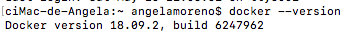
\includegraphics[width=8cm,height=8cm,keepaspectratio]{./Contenedores/Azure/10.png}
\end{nscenter}
\newline
A continuación voy a desplegar un contenedor a partir de unas imágenes de un repositorio en github que ofrece una aplicación de votos online. Para ello, clonamos el repositorio.
\newline
\begin{nscenter}
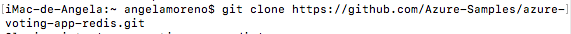
\includegraphics[width=8cm,height=8cm,keepaspectratio]{./Contenedores/Azure/11.png}
\end{nscenter}
\newline
A continuación, mostramos los contenedores que hay en ejecución.
\newline
\begin{nscenter}
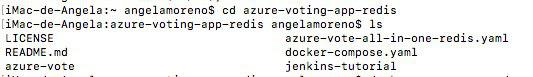
\includegraphics[width=8cm,height=8cm,keepaspectratio]{./Contenedores/Azure/12.png}
\end{nscenter}
\newline
El front de la aplicación está corriendo en localhost, en el puerto 8080. Por tanto, si vamos al explorador e intentamos acceder al puerto 8080 del localhost debería de aparecer la aplicación:
\newline
\begin{nscenter}
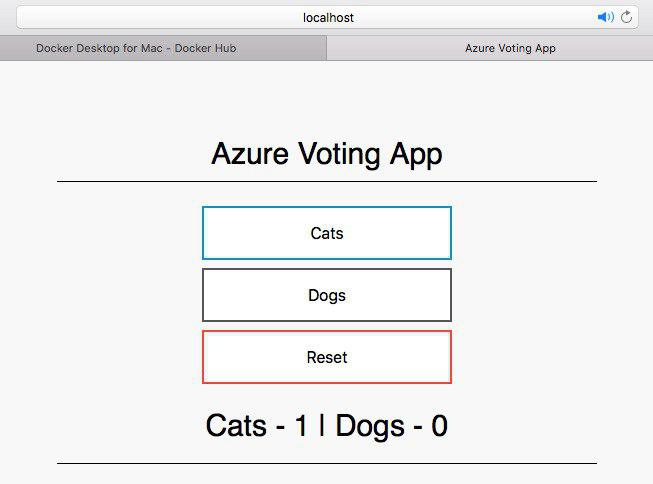
\includegraphics[width=8cm,height=8cm,keepaspectratio]{./Contenedores/Azure/13.png}
\end{nscenter}
\newline
A continuación, voy a mostrar de nuevo los contenedores que hay en ejecución:
\newline
\begin{nscenter}
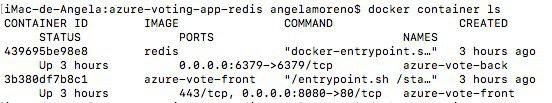
\includegraphics[width=8cm,height=8cm,keepaspectratio]{./Contenedores/Azure/14.png}
\end{nscenter}
\newline
Voy a intentar borrar uno de ellos, en concreto azure-vote-back:

\begin{nscenter}
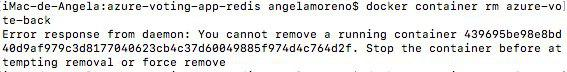
\includegraphics[width=8cm,height=8cm,keepaspectratio]{./Contenedores/Azure/15.jpg}
\end{nscenter}
\newline
Como se puede ver en la imagen, no deja borrar un contenedor que se esté ejecutando a no ser que lo paremos o que forcemos su borrado. Por tanto, fuerzo su borrado:
\newline
\begin{nscenter}
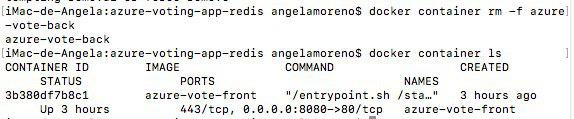
\includegraphics[width=8cm,height=8cm,keepaspectratio]{./Contenedores/Azure/16.jpg}
\end{nscenter}
\newline
Como se puede ver, el contenedor "azure-vote-back" ya no está activo, y si intentamos acceder de nuevo a la página donde está la aplicación nos vamos a encontrar con que ya no funciona:
\newline
\begin{nscenter}
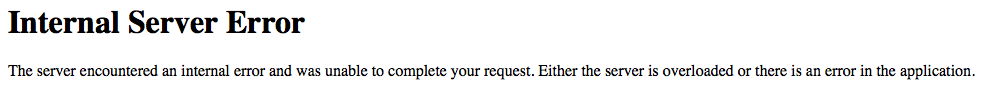
\includegraphics[width=8cm,height=8cm,keepaspectratio]{./Contenedores/Azure/17.png}
\end{nscenter}
\newpage
\subsection*{Creación de una aplicación en contenedores con Azure Web App for Containers}

App Service Linux proporciona pilas de aplicaciones predefinidas en Linux con compatibilidad con .NET, PHP y Node.js entre otros. En el ejemplo que viene a continuación se va a crear una web e implementar una imagen de GO desde Docker Hub. Para ello, voy a utilizar la CLI de Azure.

\subsubsection*{Crear un grupo de recursos}
Un grupo de recursos es un contenedor lógico en el que se implementan y administran recursos de Azure como aplicaciones web, bases de datos y cuentas de almacenamiento. \\
Para crear dicho grupo de recursos, en la CLI de Azure, se introduce la siguiente instrucción: \\
\begin{nscenter}
\noindent\rule{10cm}{0.4pt}

az group create --name miGru --location "West Europe"

\noindent\rule{10cm}{0.4pt}
\end{nscenter}
\newline
El grupo creado se llama "miGru" y tiene como localización el oeste de Europa.\\
Como respuesta a la instrucción ejecutada la CLI de Azure mostrará un JSON donde hará saber que la instrucción ha sido ejecutada correctamente y se ha creado el grupo.
\newline
\begin{nscenter}
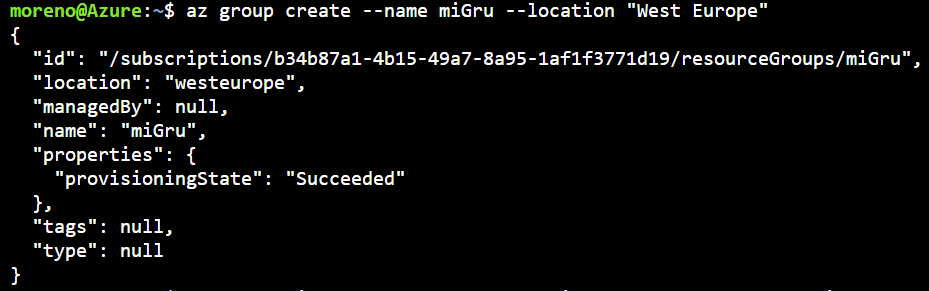
\includegraphics[width=8cm,height=8cm,keepaspectratio]{./Contenedores/Azure/2.png}
\end{nscenter}
\subsubsection*{Crear un plan de Azure App Service}
Se crea un plan App Service a través de la CLI de Azure:
\begin{nscenter}
\noindent\rule{10cm}{0.4pt}

az appservice plan create --name miPlan \\--resource-group miGru --ski B1 --is-linux

\noindent\rule{10cm}{0.4pt}
\end{nscenter}
\newline
El plan creado se llama miPlan y pertenece al grupo creado anteriormente.\\
Con el valor "B1" asignamos un plan de tarifa básico y con "--is-linux" determinamos que es un contenedor Linux.
\newline
\begin{nscenter}
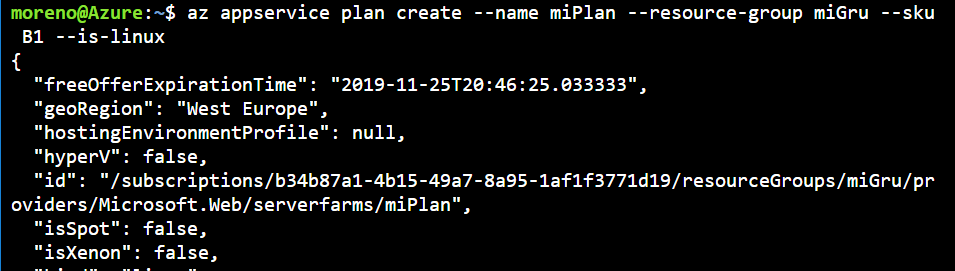
\includegraphics[width=8cm,height=8cm,keepaspectratio]{./Contenedores/Azure/3.png}
\end{nscenter}
\subsubsection*{Creación de una aplicación web}
Ahora, a través de la CLI, se va a crear una aplicación web.
\newline
\begin{nscenter}
\noindent\rule{10cm}{0.4pt}

az webapp create --resource-group miGru --plan miPlan --name nombreApplication --deployment-container-image-name microsoft/azure-appservices-go-quickstart

\noindent\rule{10cm}{0.4pt}
\end{nscenter}
\newline
Con el comando "--deployment-container-image-name" apuntamos a la imagen pública de Docker Hub. \\
\begin{nscenter}
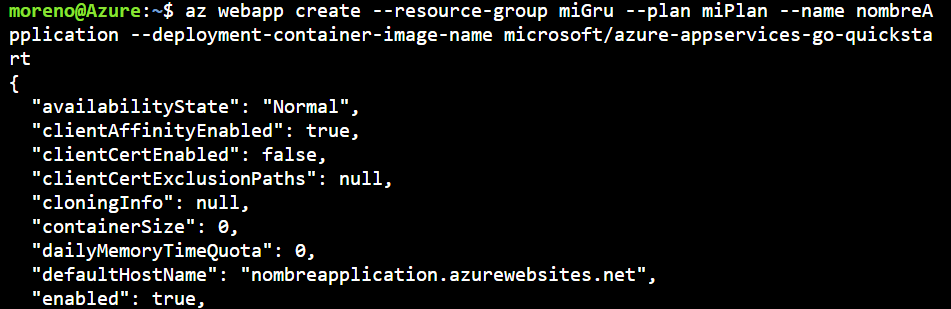
\includegraphics[width=8cm,height=8cm,keepaspectratio]{./Contenedores/Azure/4.png}
\end{nscenter}
\subsubsection*{Navegación hasta la aplicación}
Debido a que el nombre elegido pata el nombre de la aplicación web es "nombreApplication", la URL que deberemos de introducir en el navegador para ir a nuestra página web es la siguiente:\\
\begin{nscenter}
\noindent\rule{10cm}{0.4pt}

http:nombreapplication.azurewebsites.net/hello

\noindent\rule{10cm}{0.4pt}
\newline
\end{nscenter}
Mostrándose en el navegador lo siguiente:
\newline
\begin{nscenter}
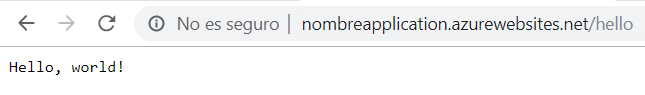
\includegraphics[width=8cm,height=8cm,keepaspectratio]{./Contenedores/Azure/5.png}
\end{nscenter}
\newpage
\subsection*{Ejecución a petición de aplicaciones de contenedor en Azure Container Instances}

En este apartado se va a usar la CLI de Azure para implementar un contenedor de docker aislado y hacer que la aplicación esté disponible con un nombre de dominio completo.\\
\subsubsection*{Creación de un grupo de recursos}
\begin{nscenter}
\noindent\rule{10cm}{0.4pt}

az group create --name myGroup --location "west Europe"

\noindent\rule{10cm}{0.4pt}
\end{nscenter}
\subsubsection*{Creación de un contenedor}
Para crear una instancia de contenedor de la CLI de Azure hay que proporcionar un nombre al grupo de recursos, un nombre de instancia de contenedor y una imagen de contenedor de Docker. En este ejemplo se usa una pública, que empaqueta una aplicación en Node.js que sirve una página HTML estática.\\
Los contenedores se pueden exponer en Internet mediante la especificación para que se abran uno o varios puertos.\\
Mediante la etiqueta "--dnd-name-label" se le establece un valor DNS.
\begin{nscenter}
\noindent\rule{10cm}{0.4pt}

az container create --resource-group myGroup --name mycontainer --image mcr.microsoft.com/azuredocs/aci-helloworld\\ --dns-name-label acidemo --ports 80

\noindent\rule{10cm}{0.4pt}
\end{nscenter}
\newline
A continuación, comprobamos el estado:
\newline
\begin{nscenter}
\noindent\rule{10cm}{0.4pt}

az container show --resource-group myGroup --name mycontainer\\ --query "{FQDN:ipAddress.fqdn,ProvisioningState:provisioningState}" --out table
\noindent\rule{10cm}{0.4pt}
\end{nscenter}
\newline
\begin{nscenter}
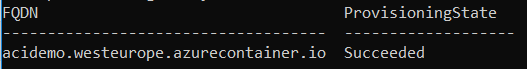
\includegraphics[width=8cm,height=8cm,keepaspectratio]{./Contenedores/Azure/6.png}
\end{nscenter}

El estado es "Succeeded", por lo que sí introducimos el FQDN en el navegador, lo que se muestra es lo siguiente:
\newline
\begin{nscenter}
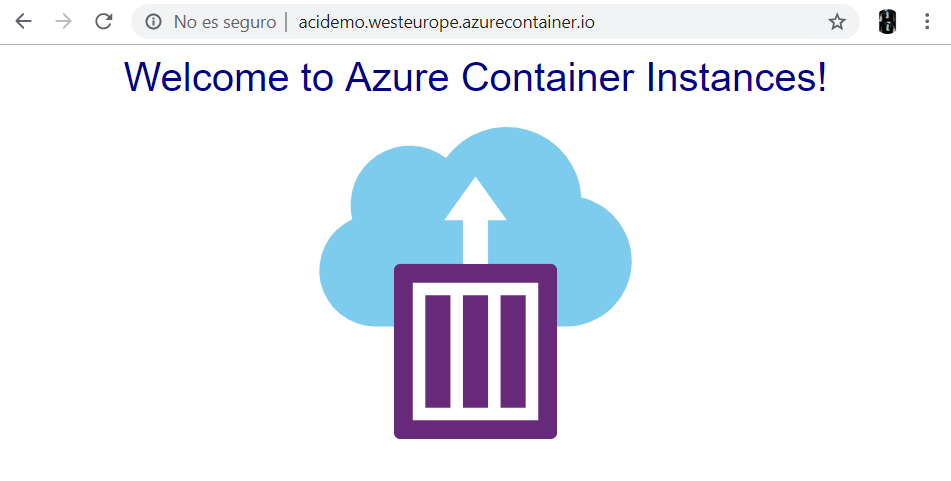
\includegraphics[width=8cm,height=8cm,keepaspectratio]{./Contenedores/Azure/7.png}
\end{nscenter}

\subsubsection*{Extraer los registros del contenedor}

\begin{nscenter}
\noindent\rule{10cm}{0.4pt}

az container logs --resource-group myGroup --name mycontainer

\noindent\rule{10cm}{0.4pt}
\end{nscenter}
\newline
\begin{nscenter}
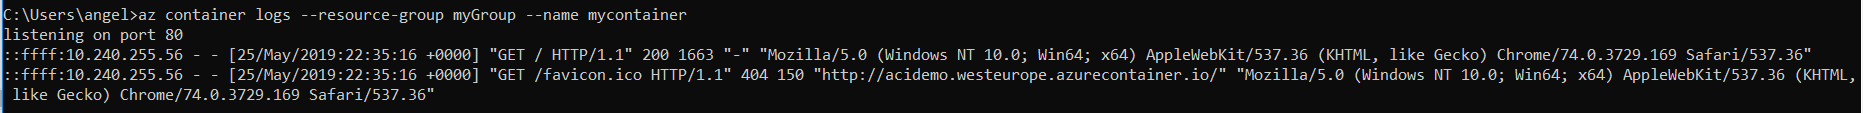
\includegraphics[width=12cm,height=12cm,keepaspectratio]{./Contenedores/Azure/8.png}
\end{nscenter}
\newline
Se muestran los registros del contenedor, addemás de las solicitudes HTTP GET generadas al ver la aplicación en el explorador.
\newpage
\subsection*{Creación de un registro de Docker privado en Azure Container Registry}

Para esta subsección, al contrario que en todas las anteriores desarrolladas, he tenido que instalarme la CLI de Azure, no pudiendo utilizar la versión Cloud.

\subsubsection*{Crear un grupo de recursos}
\begin{nscenter}
\noindent\rule{10cm}{0.4pt}

az group create --name miGrupo --location "West Europe"

\noindent\rule{10cm}{0.4pt}
\end{nscenter}

\subsubsection*{Crear un registro de contenedor}
\begin{nscenter}
\noindent\rule{10cm}{0.4pt}

az acr create --resource-group miGrupo --name miRegistro0024 --sku Basic

\noindent\rule{10cm}{0.4pt}
\end{nscenter}

\subsubsection*{Insertar la imagen en el registro}
\begin{nscenter}


\noindent\rule{10cm}{0.4pt}

az acr login --name miRegistro0024

\noindent\rule{10cm}{0.4pt}
\end{nscenter}

En este paso, sin embargo, se muestra lo siguiente por la CLI:
\newline
\begin{nscenter}
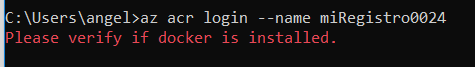
\includegraphics[width=8cm,height=8cm,keepaspectratio]{./Contenedores/Azure/9.png}
\end{nscenter}
\newline
Tal y como se puede ver, no se puede seguir adelante sin tener Docker instalado.\\
El problema en este caso es que, al intentar instalar Docker una de las restricciones es que se debe de tener Windows 10 Pro, el cual yo no tengo. \\
Por tanto, se va a repetir todo el proceso desde el ordenador cuyo sistema operativo es macOS Sierra y donde sí que pude instalar Docker. \\
Antes de insertar imágenes hay que iniciar sesión en la instancia de Azure container Registry especificando el nombre del contenedor creado. En mi caso, y debido al cambio de ordenador, el nuevo nombre del registro es 'registromoreno'. \\
También ejecuto un 'az acr show' para obtener el nombre del servidor de inicio de sesión completo de la instancia de Azure Container Registry.
\newline
\begin{nscenter}
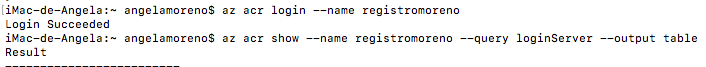
\includegraphics[width=8cm,height=8cm,keepaspectratio]{./Contenedores/Azure/51.png}
\end{nscenter}
\newline
A continuación se muestra la lista de imágenes locales con el comando 'docker images' y podemos que aparece 'aci-tutorial-app', que es la imagen creada en apartados anteriores.
\newline
\begin{nscenter}
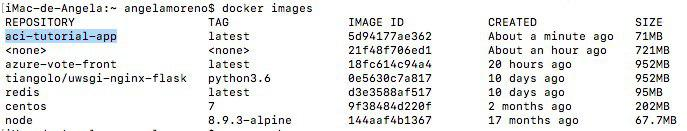
\includegraphics[width=8cm,height=8cm,keepaspectratio]{./Contenedores/Azure/18.jpg}
\end{nscenter}
\newline
Como siguiente paso etiquetamos la imagen aci-tutorial-app.
\newline
\begin{nscenter}
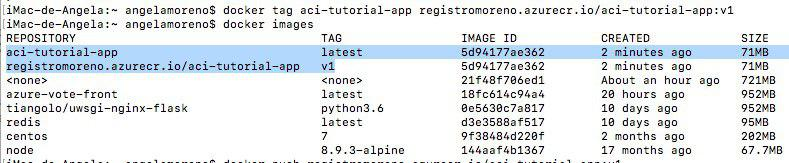
\includegraphics[width=8cm,height=8cm,keepaspectratio]{./Contenedores/Azure/19.jpg}
\end{nscenter}
\subsubsection*{Inserción de imágenes en Azure Container Registry}
Ahora que se ha etiquetado la imagen con el nombre del servidor de inicio de sesión completo, se puede insertar en el registro con el comando 'docker push'.
\newline
\begin{nscenter}
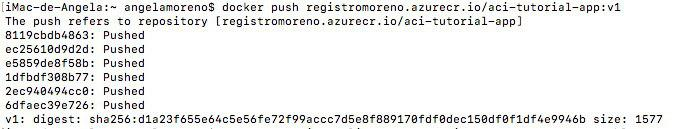
\includegraphics[width=8cm,height=8cm,keepaspectratio]{./Contenedores/Azure/20.jpg}
\end{nscenter}
\subsubsection*{Lista de imágenes en Azure Container Registry}
Ahora ejecuto el comando 'az acr repository list' para ver si la imagen se ha insertado correctamente. Y por último, con el comando 'az acr repository show-tags' hago que se imprima la etiqueta de la imagen.
\newline
\begin{nscenter}
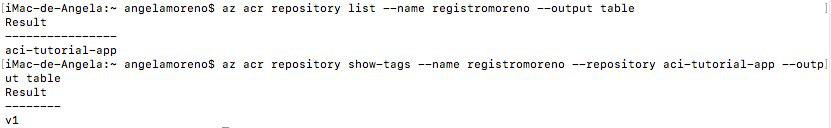
\includegraphics[width=8cm,height=8cm,keepaspectratio]{./Contenedores/Azure/21.jpg}
\end{nscenter}
\newpage
\section*{AWS}
Con respecto a AWS, los casos de uso de los contenedores son: microservicios, para aislar procesos; procesamiento de lotes, para arrancarlos con rapidez y escalarlos de forma dinámica dependiendo de la demanda; aplicaciones híbridas, puesto que los contenedores le permiten administrar de un modo uniforme la forma en que se implementa el código y la migración de aplicaciones a la nube, puesto que los contenedores facilitan la tarea de empaquetar aplicaciones enteras y trasladarlas a la nube sin cambiar nada del código. También permiten diseñar plataformas para que los desarrolladores no tengan que administrar infraestructuras y aprendizaje automático.
A su vez, Amazon tiene diferentes servicios: Amazon ECR, Amazon ECS, Amazon EKS, AWS Fargate y Amazon EC2.


\newpage
\subsection*{Amazon ECR}
Servicio para almacenar imágenes en contenedores. Los desarrolladores pueden usar la CLI de Docker para diseñar, insertar, extraer y administrar imágenes.

\subsubsection*{Componentes}
Registro: Cada cuenta de AWS recibe un registro de Amazon ECR donde puede crear repositorios de imágenes y guardar imágenes en ellos.\\
Token de autorización: Debe autenticar el cliente de Docker en los registros de Amazon ECR cono usuario de AWS para que dicho cliente pueda insertar y extraer imágenes. A través del comando get-login de la AWS CLI se proporcionan credenciales para pasarlas al Docker.\\
Repositorio: Contiene las imágenes de Docker.\\
Política sobre repositorios: Se puede controlar el acceso a los repositorios e imágenes. \\
Imagen: Se puede insertar y extraer imágenes de Docker en los repositorios y usarlas localmente.
\subsubsection*{Introducción a Amazon ECR}
En este apartado nos van a enseñar a crear un repositorio en la consola de Amazon ECR. Para ello, abro la consola de Amazon ECR y selecciono el nombre que va a tener el primer repositorio, que va a ser angelamoreno. \\
Una vez introducido el nombre y creado el repositorio, AWS muestra la siguiente interfaz:
\newline
\begin{nscenter}
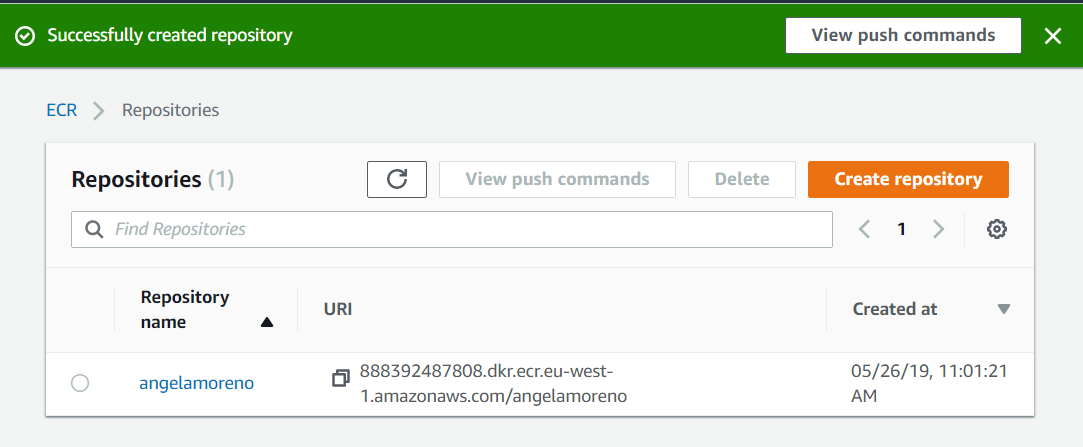
\includegraphics[width=8cm,height=8cm,keepaspectratio]{./Contenedores/AWS/27.png}
\end{nscenter}
\subsubsection*{Creación, etiquetado y envío de imágenes Docker}
Lo primero que hay que hacer es instalar la CLI de AWS. Una vez hecho, ejecutamos el comando 'aws configure'. \\
Al ejecutar el comando 'aws configure' nos va a pedir que introduzcamos una clave de acceso ID, una contraseña de acceso, el nombre de la región en la que se creó el repositorio y el tipo de output por defecto. \\
Para obtener el ID y la contraseña hay que ir al IAM Management Console de AWS, al apartado de Usuarios y generar una clave de acceso. El ID y la contraseña generadas en el momento son las que tenemos que introducir en la CLI de AWS. \\
A continuación, ejecutando el comando 'docker login' se pedirán los credenciales de Docker. \\
\newline
\begin{nscenter}
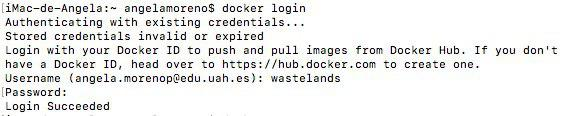
\includegraphics[width=8cm,height=8cm,keepaspectratio]{./Contenedores/AWS/17.jpg}
\end{nscenter}
\newline
A partir de ese momento, a través de los comandos 'docker tag' y 'docker push' podremos insertar imágenes en el repositorio creado.

\newpage
\subsection*{Introducción a Amazon ECS}
Amazon Elastic Container (Amazon ECS) es un servicio de administración de contenedores muy escalable y rápido que facilita la tarea de ejecutar, detener y gestionar contenedores de Docker en un clúster de instancias de Amazon EC2.\\
Para configurar un ECS hay que seguir los siguientes pasos: \\
Primero creamos una cuenta de AWS en http://aws.amazon.com/ y después darnos a nosotros mismos el permiso de ser administradores.
\begin{nscenter}
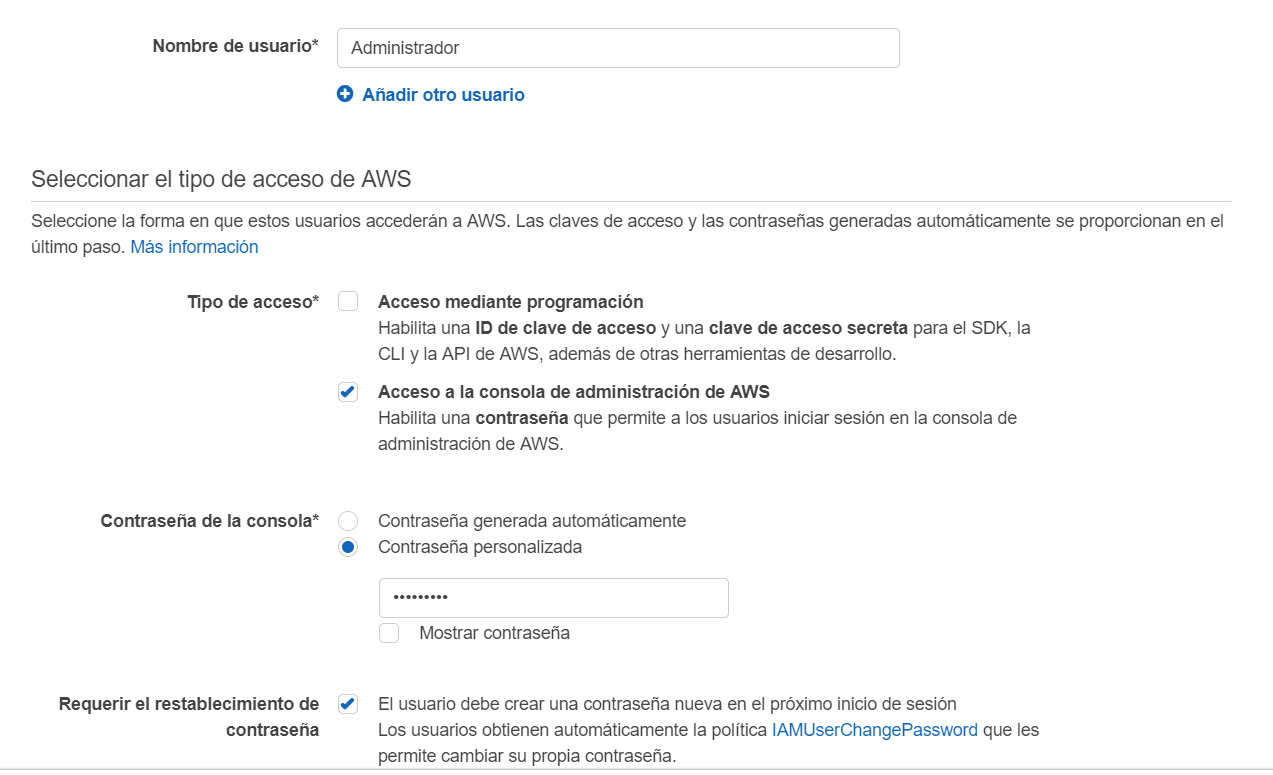
\includegraphics[width=8cm,height=8cm,keepaspectratio]{./Contenedores/AWS/28.png}
\end{nscenter}
\newline
A continuación hay que crear un grupo, el cual va a tener de nombre Administrators donde, al usuario previamente creado, se le asignan unas políticas. \\
Una vez asignadas y creado el usuario, la pantalla es la siguiente: 
\newline
\begin{nscenter}
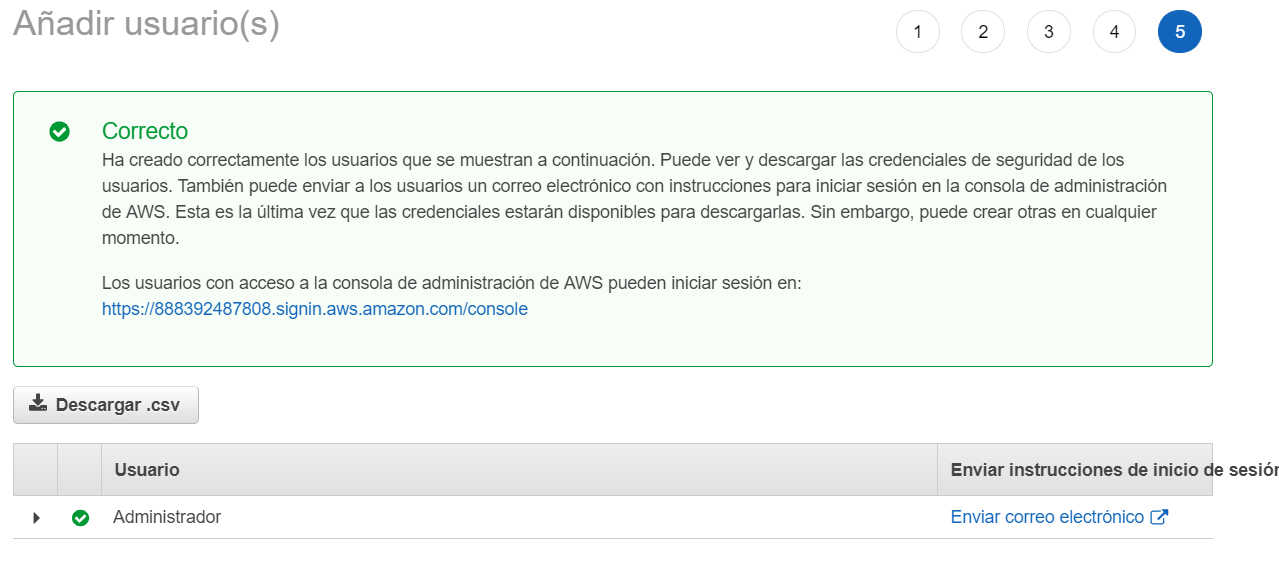
\includegraphics[width=8cm,height=8cm,keepaspectratio]{./Contenedores/AWS/29.png}
\end{nscenter}
\newline
Una vez creado el usuario, nos piden que accedamos a él.
\newline
\begin{nscenter}
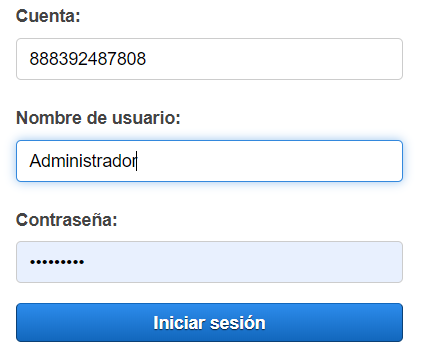
\includegraphics[width=8cm,height=8cm,keepaspectratio]{./Contenedores/AWS/30.png}
\end{nscenter}
\newline
Tal y como se seleccionó en las opciones al crear el usuario, al iniciar sesión, el administrador tiene que cambiar la contraseña antigua por una nueva.\newline
\newline
\begin{nscenter}
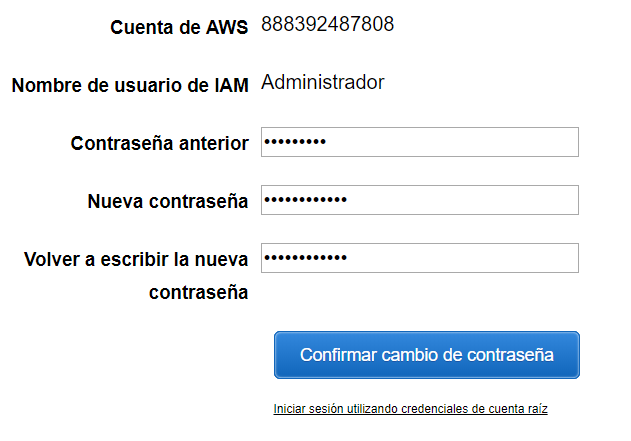
\includegraphics[width=8cm,height=8cm,keepaspectratio]{./Contenedores/AWS/31.png}
\end{nscenter}
\newline
Después de esto, ya podemos crear una VPC (nube virtual privada). \\
Para ello, lo que hay que hacer es abrir la consola de Amazon VPC y lanzar el asistente de VPC, la cual tenga una única subred pública. También hay que ponerle un nombre, el cual va a ser angelamoreno. Una vez que se ha creado, la pantalla que nos muestra AWS es la siguiente: 
\newline
\begin{nscenter}
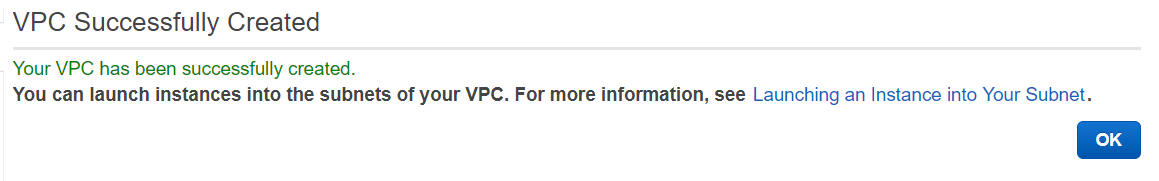
\includegraphics[width=8cm,height=8cm,keepaspectratio]{./Contenedores/AWS/32.png}
\end{nscenter}
\newline
\newpage
\subsection*{Introducción a Amazon EKS}
Amazon Elastic Container Service for Kubernetes (Amazon EKS) es un servicio administrado que permite ejecutar Kubernetes AWS sin necesidad de crear ni mantener su propio plano de control de Kubernetes. Kubernetes es un sistema de código abierto para automatizar la implementación, escalado y administración de las aplicaciones en contenedores. \\
Amazon EKS detecta y reemplaza automáticamente las instancias del plano de control en mal estado, y proporciona actualizaciones de versiones y parches automatizados para ellas. También integra numerosos servicios AWS para ofrecer escalabilidad y seguridad a las aplicaciones, como IAM para la autenticación, Amazon VPC para el aislamiento...
\subsubsection*{Creación del clúster de Amazon EKS y los nodos de trabajo}
Para hacer esta parte de la práctica he tenido que instalar eksctl y kubectl. \\
Inicialmente creamos el clúster de Amazon EKS y los nodos de trabajo con el siguiente comando:
\newline
\begin{nscenter}
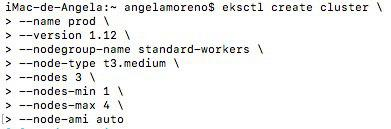
\includegraphics[width=8cm,height=8cm,keepaspectratio]{./Contenedores/AWS/22.jpg}
\end{nscenter}
\subsubsection*{Lanzar aplicación de libro de invitados}
Para lanzar la aplicación de libro de invitados hay que crear el controlador de replicación maestro Redis, además de crear el servicio, el controlador de replicación esclavo, el servicio esclavo Redis, también crear el controlador de replicación de guestbook y el servicio guestbook.
\newline
\begin{nscenter}
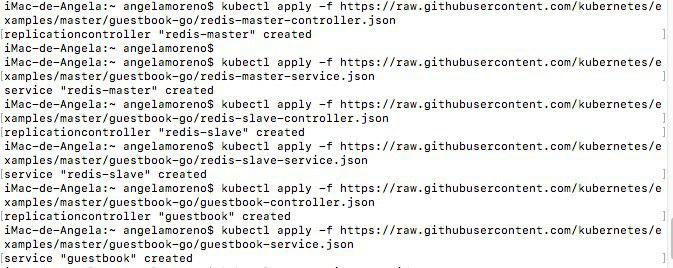
\includegraphics[width=8cm,height=8cm,keepaspectratio]{./Contenedores/AWS/23.jpg}
\end{nscenter}
\newline
Por último, hay que mirar la dirección externa del servicio guestbook a través del comando 'kubectl get services -o wide'.
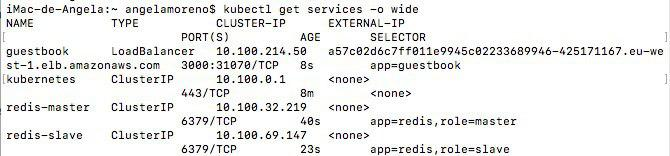
\includegraphics[width=8cm,height=8cm,keepaspectratio]{./Contenedores/AWS/2.jpg}
\subsubsection*{Uso de Heml con Amazon EKS}
Para esta parte de la práctica hay que crear, a través de la consola, un servidor y un cliente que se conecta a dicho servidor creado.
\newline
\begin{nscenter}
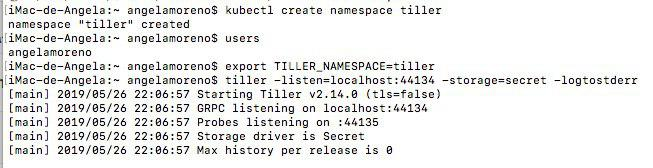
\includegraphics[width=8cm,height=8cm,keepaspectratio]{./Contenedores/AWS/24.jpg}
\end{nscenter}
\newline
En el terminal del servidor de tiller se establece la variable de entorno TILLER NAMESPACE y a continuación se inicia el servidor. \\
A continuación, en la terminal de cliente helm, establecemos la variable de entorno HELM HOST:44134 y nos conectamos al servidor.
\newline
\begin{nscenter}
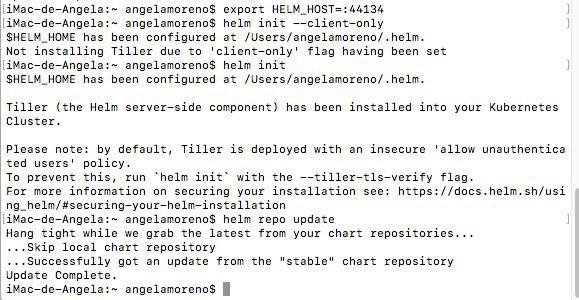
\includegraphics[width=8cm,height=8cm,keepaspectratio]{./Contenedores/AWS/25.jpg}
\end{nscenter}
\newpage
\subsection*{Introducción a Amazon EC2}
Amazon Elastic Compute Cloud (amazon EC2) proporciona capacidad de computación escalable en la nuble de Amazon Web Services (AWS) El uso de Amazon EC2 elimina la necesidad de invertir en hardware.
\subsubsection*{Lanzar una instancia}
Para crear una instancia hay que hacer uso de la consola de Amazon EC2. \\
Una vez que se ha seleccionado el lanzar una instancia, hay que elegir una imagen de máquina de Amazon (AMI), que en mi caso ha sido la Windows Server 2016 Base, como se muestra a continuación. Ésta AMI está marcada como Free tier eligible.
\newline
\begin{nscenter}
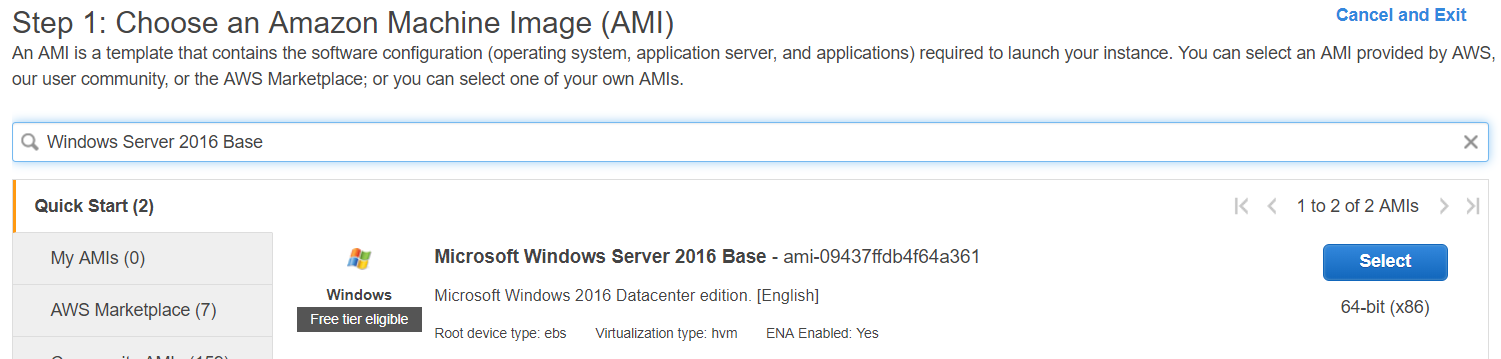
\includegraphics[width=8cm,height=8cm,keepaspectratio]{./Contenedores/AWS/33.png}
\end{nscenter}
\newline
A continuación hay que elegir un tipo de instancia, quedándonos con la t2.micro que es la que viee por defecto; después de esto, revisamos y lanzamos.
\newline
\begin{nscenter}
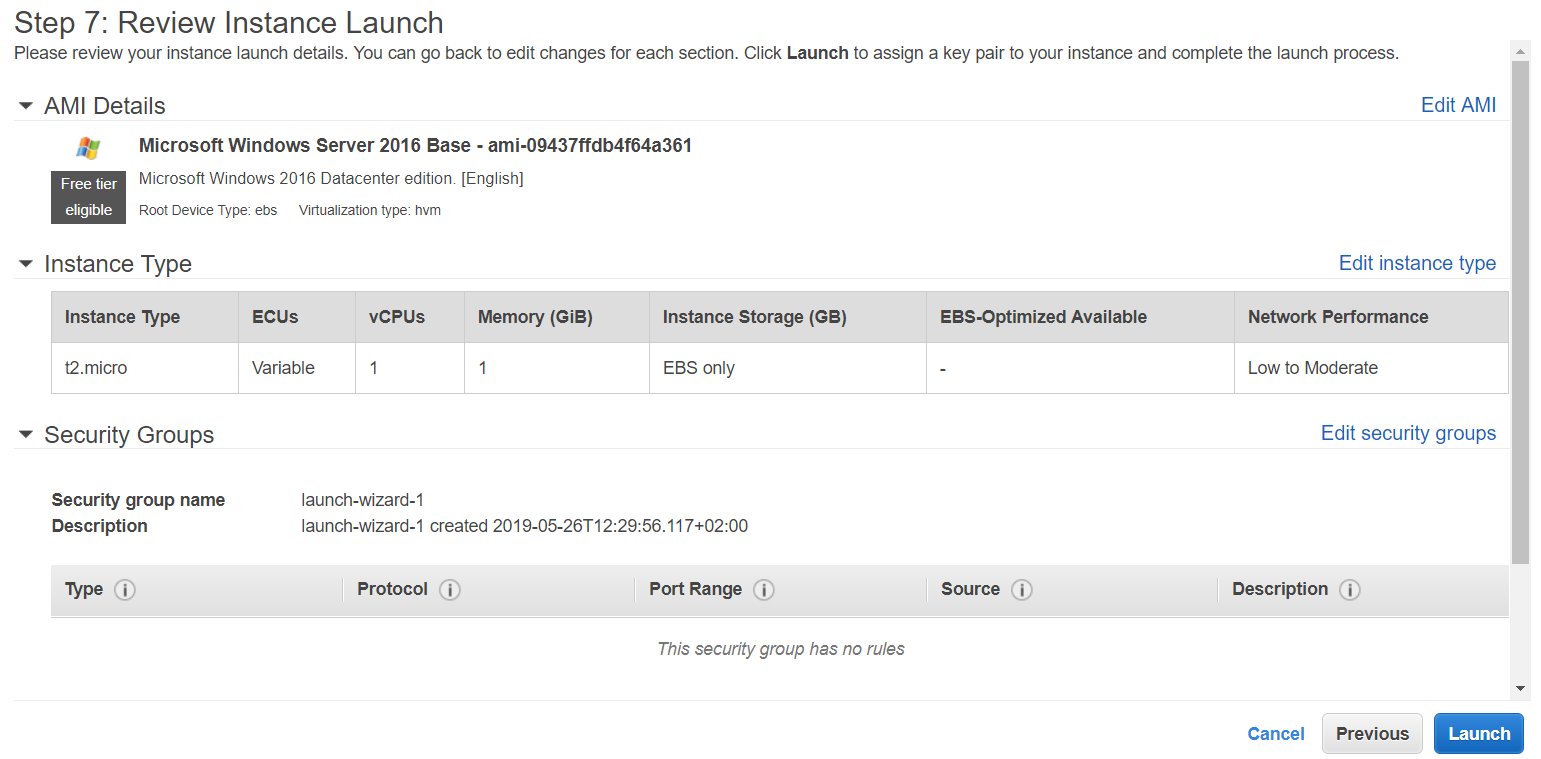
\includegraphics[width=8cm,height=8cm,keepaspectratio]{./Contenedores/AWS/34.png}
\end{nscenter}
\newline
Al ir a lanzar la instancia, nos hace descargarnos un par de llaves, a las cuales les tienes que asignar un nombre, siendo angelamorenokey el elegido. Descarga un archivo que se corresponde con esas llaves.
\newline
\begin{nscenter}
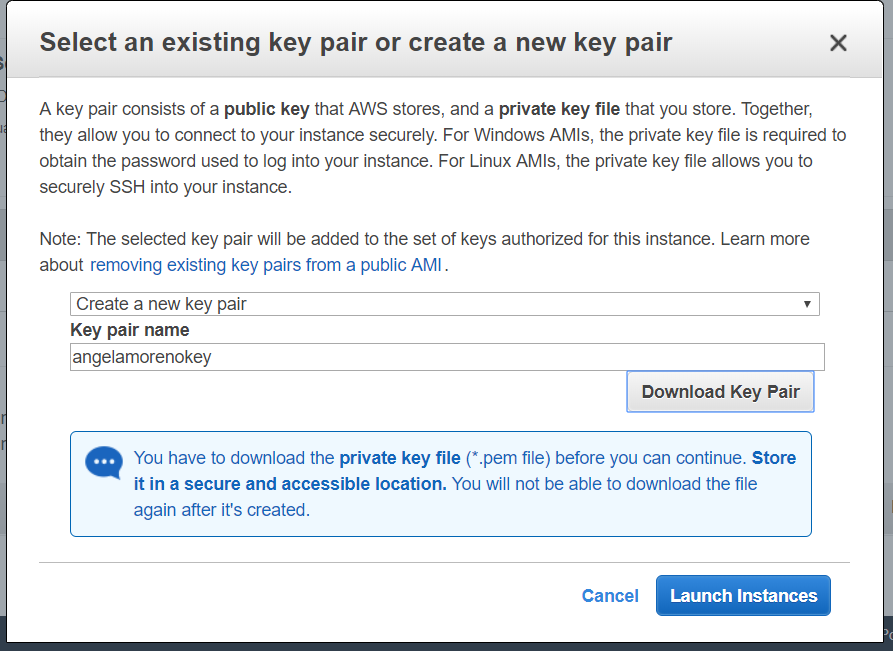
\includegraphics[width=8cm,height=8cm,keepaspectratio]{./Contenedores/AWS/35.png}
\end{nscenter}
\newline
Por último, si le damos a lanzar, la instancia queda lanzada y, a partir de ese momento, podemos conectarnos a ella.
\newline
\begin{nscenter}
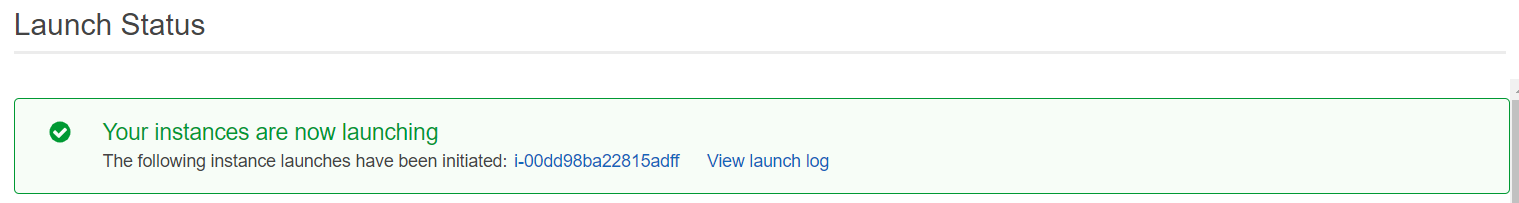
\includegraphics[width=8cm,height=8cm,keepaspectratio]{./Contenedores/AWS/36.png}
\end{nscenter}
\newline
\subsubsection*{Conectarnos a la instancia}

Para conectarnos a la instancia tenemos que volver a hacer uso de Amazon EC2, seleccionar la instancia creada anteriormente y conectarnos a ella.
\newline
\begin{nscenter}
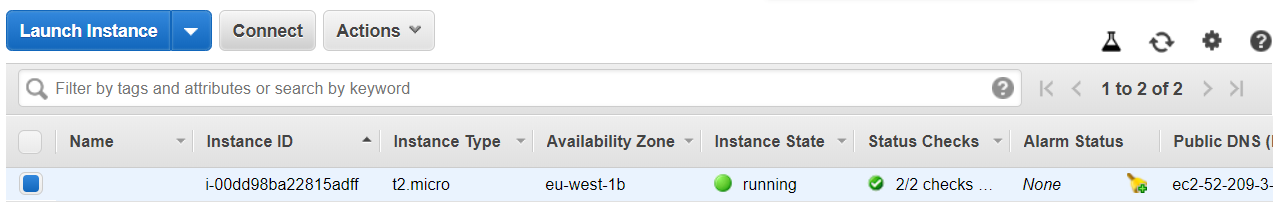
\includegraphics[width=8cm,height=8cm,keepaspectratio]{./Contenedores/AWS/37.png}
\end{nscenter}
\newline
Una vez que hayamos seleccionado el conectarnos a la instancia recién creada, AWS nos va a pedir que carguemos el archivo descargado previamente que contiene las dos llaves, el cual guardé bajo el nombre de angelamorenokey, que tiene formato .pem.
\newline
\begin{nscenter}
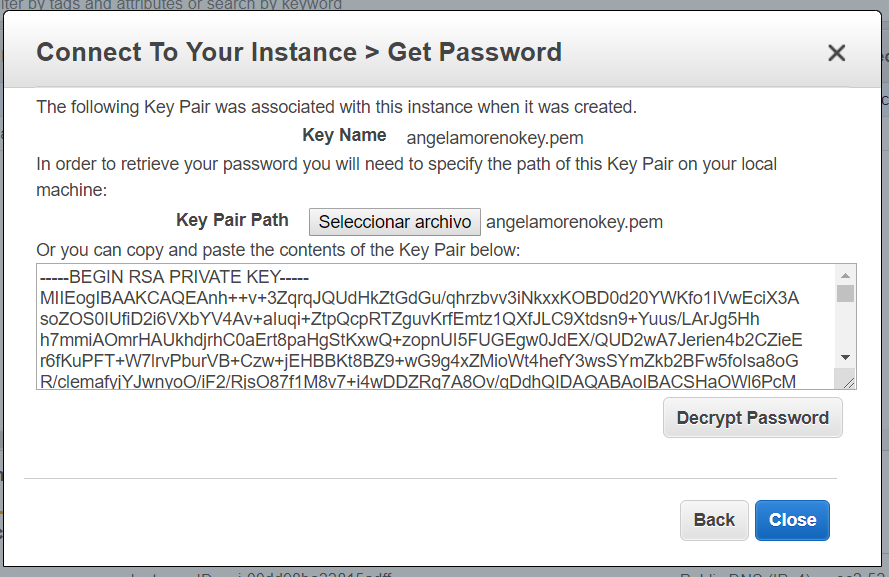
\includegraphics[width=8cm,height=8cm,keepaspectratio]{./Contenedores/AWS/38.png}
\end{nscenter}
\newline
Una vez cargado y al hacer click sobre 'Decrypt Password' podemos ver la contraseña generada resultante de subir dicho archivo .pem, correspondiente al usuario 'Administrador' que creamos anteriormente. 
\newline
\begin{nscenter}
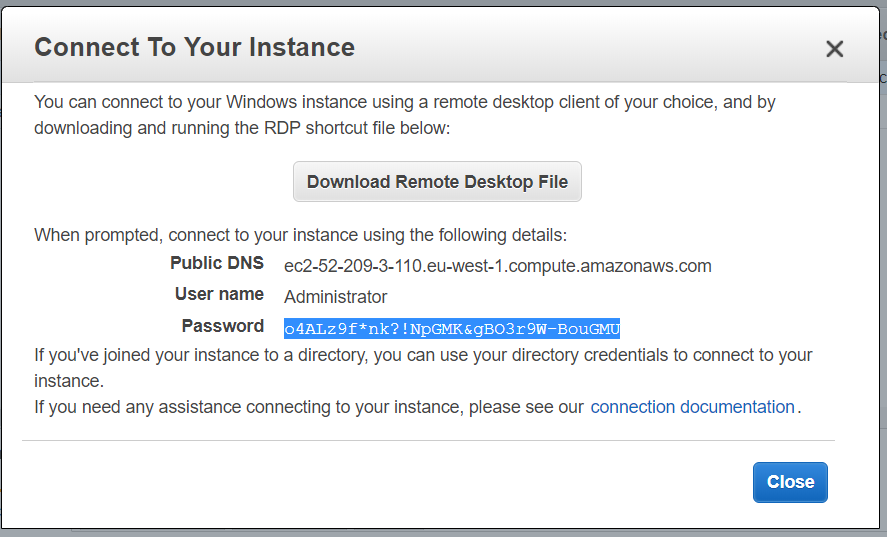
\includegraphics[width=8cm,height=8cm,keepaspectratio]{./Contenedores/AWS/39.png}
\end{nscenter}
\newline
Al hacer click sobre 'Download Remote Desktop File' se descarga un .rdp que, al ejecutarlo, va a permitir que nos conectemos a la instancia creada.
\newline
\begin{nscenter}
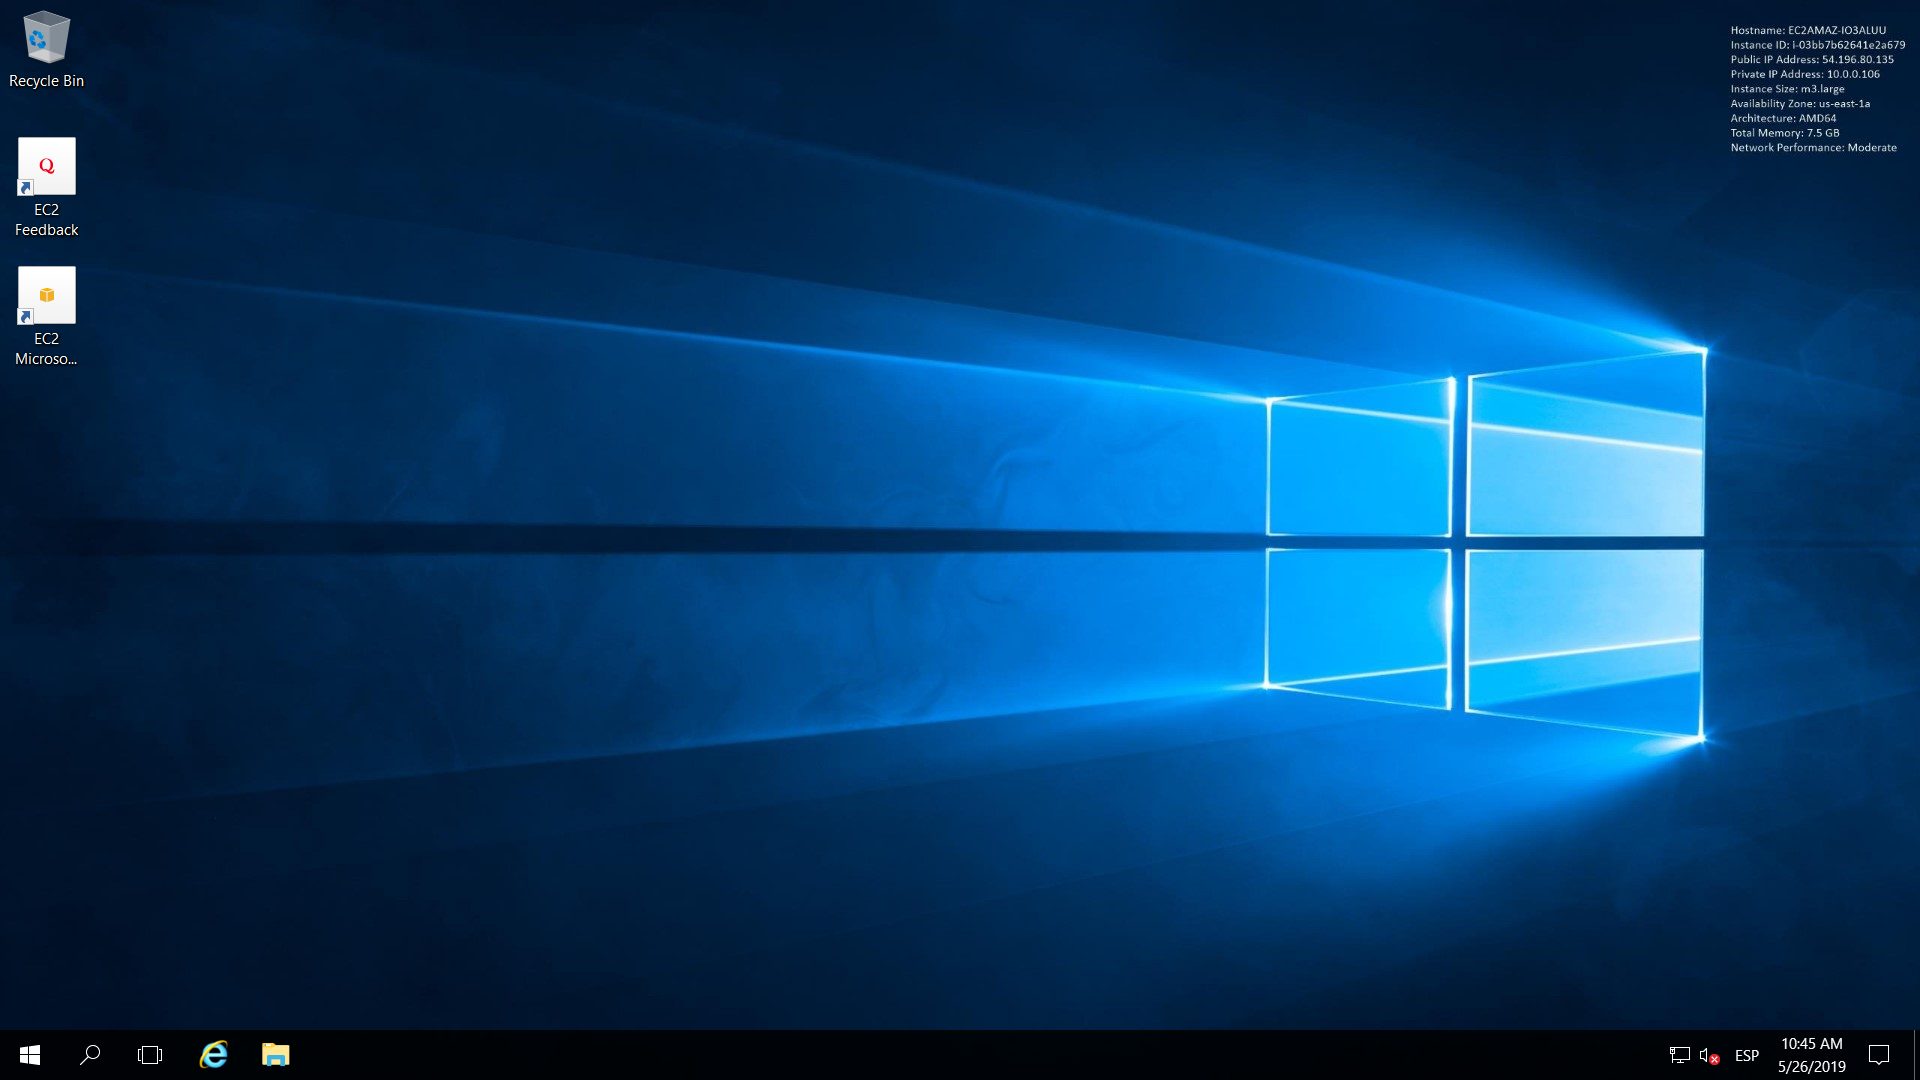
\includegraphics[width=8cm,height=8cm,keepaspectratio]{./Contenedores/AWS/41.png}
\end{nscenter}
\newline
Una vez que hayamos terminado con la instancia, tal y comos e indica en la guía proporcionada por AWS, hay que borrarla.
\newline
\begin{nscenter}
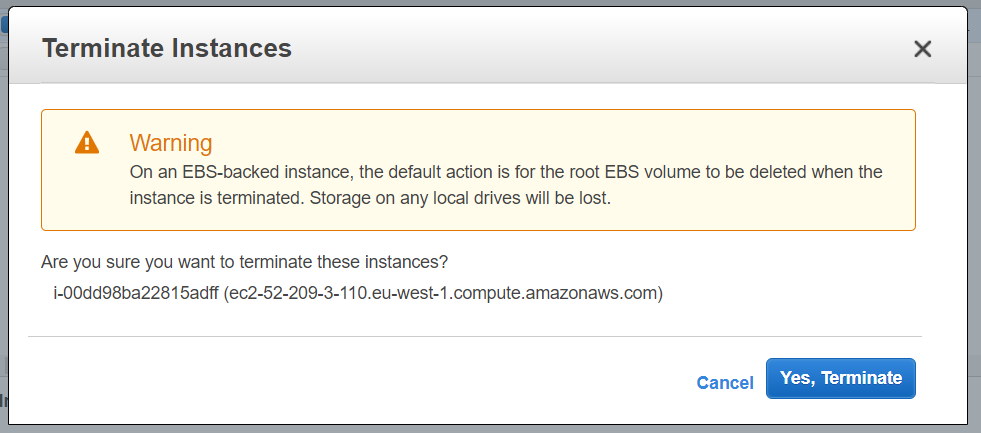
\includegraphics[width=8cm,height=8cm,keepaspectratio]{./Contenedores/AWS/42.png}
\end{nscenter}

\newpage
\subsection*{Implementar primer contenedor}
En este primer apartado, en AWS te permiten crear un primer contenedor.
\newline
\begin{nscenter}
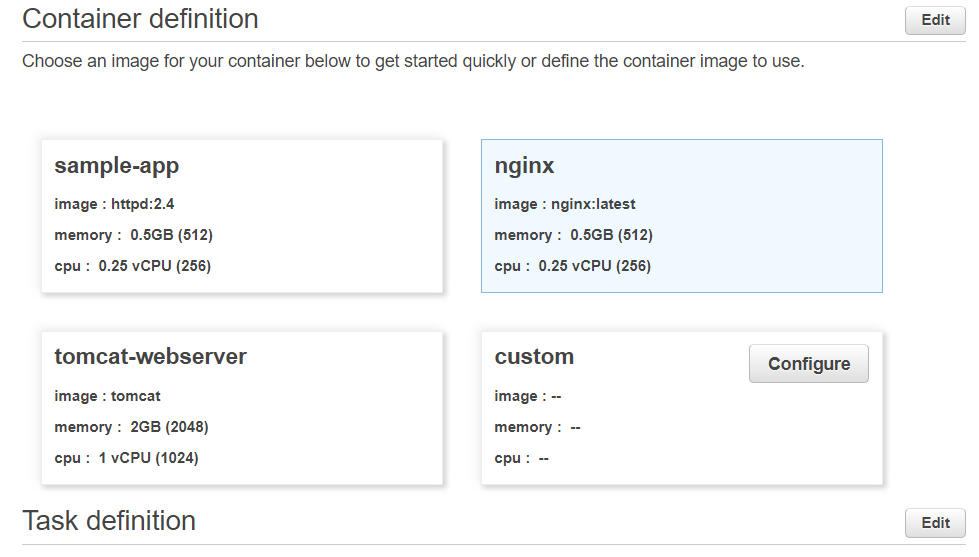
\includegraphics[width=8cm,height=8cm,keepaspectratio]{./Contenedores/AWS/18.png}
\end{nscenter}
\newline
También tienes que especificar el nombre del servicio y en qué puerto funcionará, entre otros.\\
Una vez especificados las características de este primer contenedor, AWS lo crea.
\newline
\begin{nscenter}
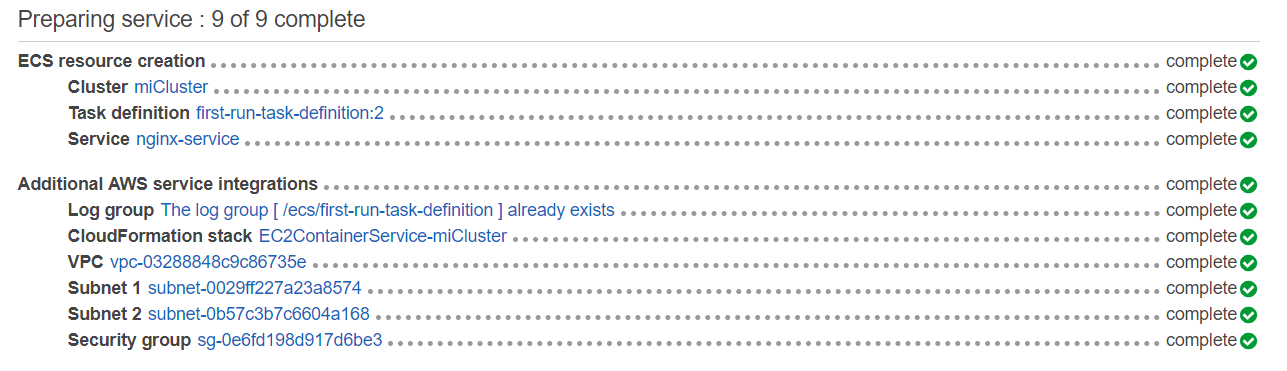
\includegraphics[width=8cm,height=8cm,keepaspectratio]{./Contenedores/AWS/19.png}
\end{nscenter}
\newline
\begin{nscenter}
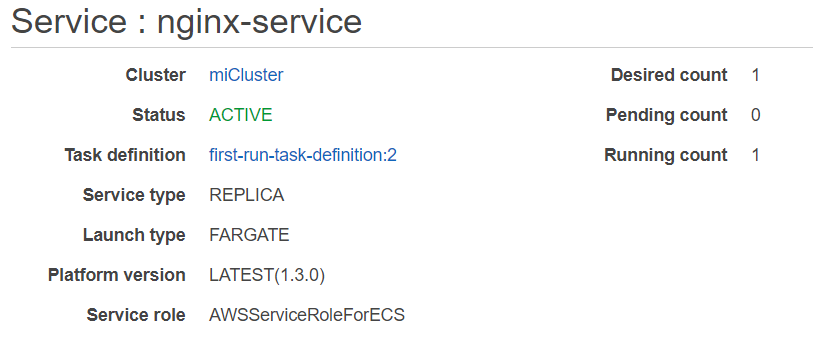
\includegraphics[width=8cm,height=8cm,keepaspectratio]{./Contenedores/AWS/20.png}
\end{nscenter}
\newpage
\subsection*{Crear una página web estática utilizando Amazon S3 y AWS Cloud 9}
Después de haber seleccionado mi localización, hay que acceder al servicio "Cloud9" desde la consola AWS, que es una nube para diseñar y depurar código.\\
Lo primero que hay que hacer, una vez hayamos accedido a la página que proporciona AWS de Cloud 9 es crear nuestro espacio de trabajo.
\newline
\begin{nscenter}
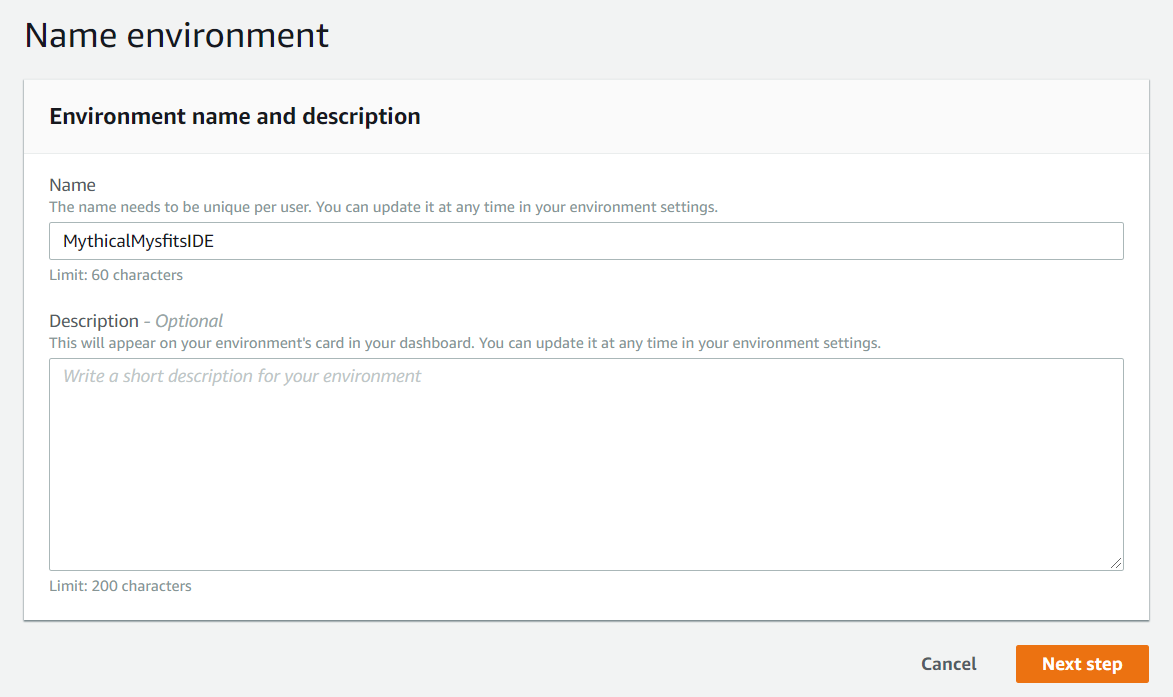
\includegraphics[width=8cm,height=8cm,keepaspectratio]{./Contenedores/AWS/21.png}
\end{nscenter}
\newline
Le he puesto "MythicalMysfitsIDE" como nombre al grupo de trabajo tal y como se muestra o indica en las instrucciones de AWS.
\newline
\begin{nscenter}
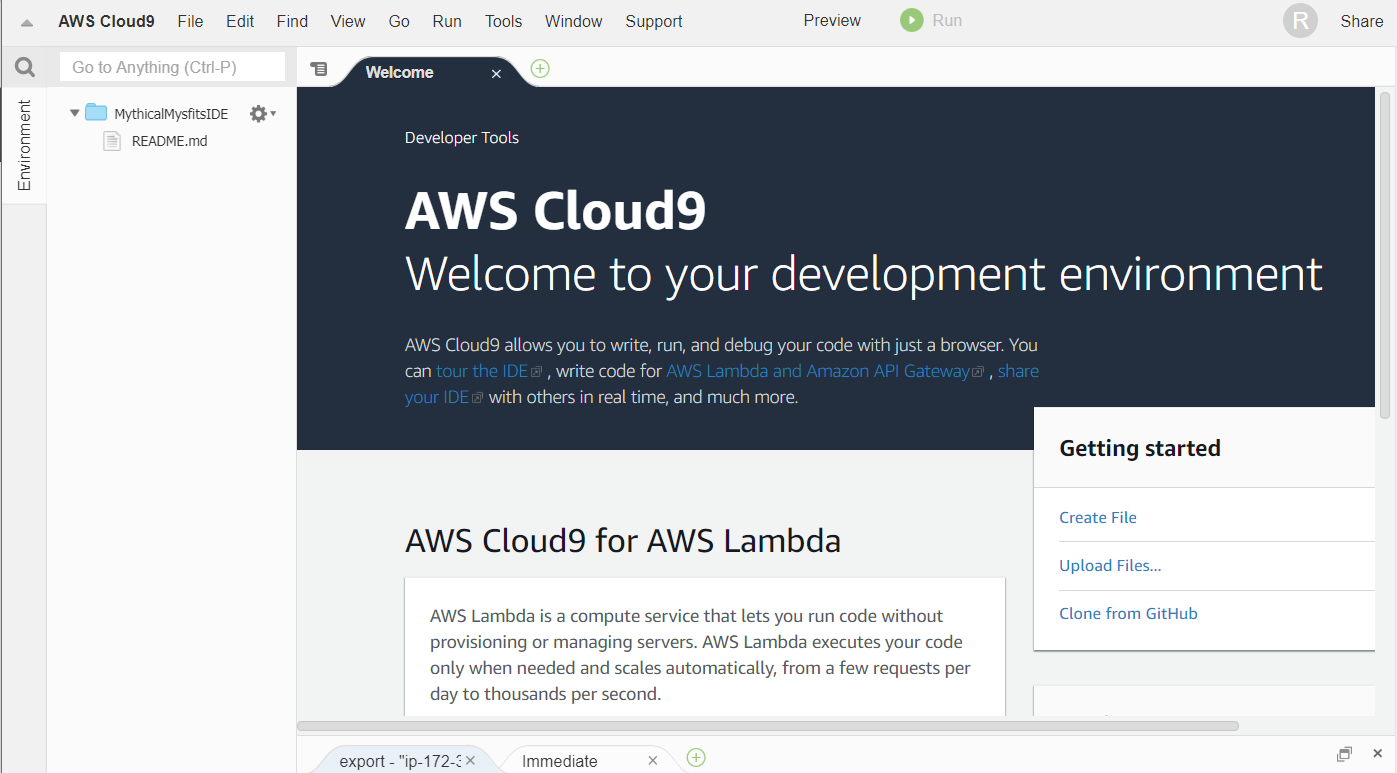
\includegraphics[width=8cm,height=8cm,keepaspectratio]{./Contenedores/AWS/22.png}
\end{nscenter}
\newline
Tal y como se muestra en la imagen, el espacio de trabajo se ha creado correctamente.\\
Piden inicialmente que clonemos el repositorio existente a través de la línea de comandos que está al final de la página previamente mostrada. Para ello, utilizo el siguiente comando:
\begin{nscenter}


\noindent\rule{10cm}{0.4pt}

git clone -b python https://github.com/aws-samples/aws-modern-application-workshop.git

\noindent\rule{10cm}{0.4pt}
\end{nscenter}

Una vez clonado, podemos ver que los archivos contenidos han cambiado.
\newline
\begin{nscenter}
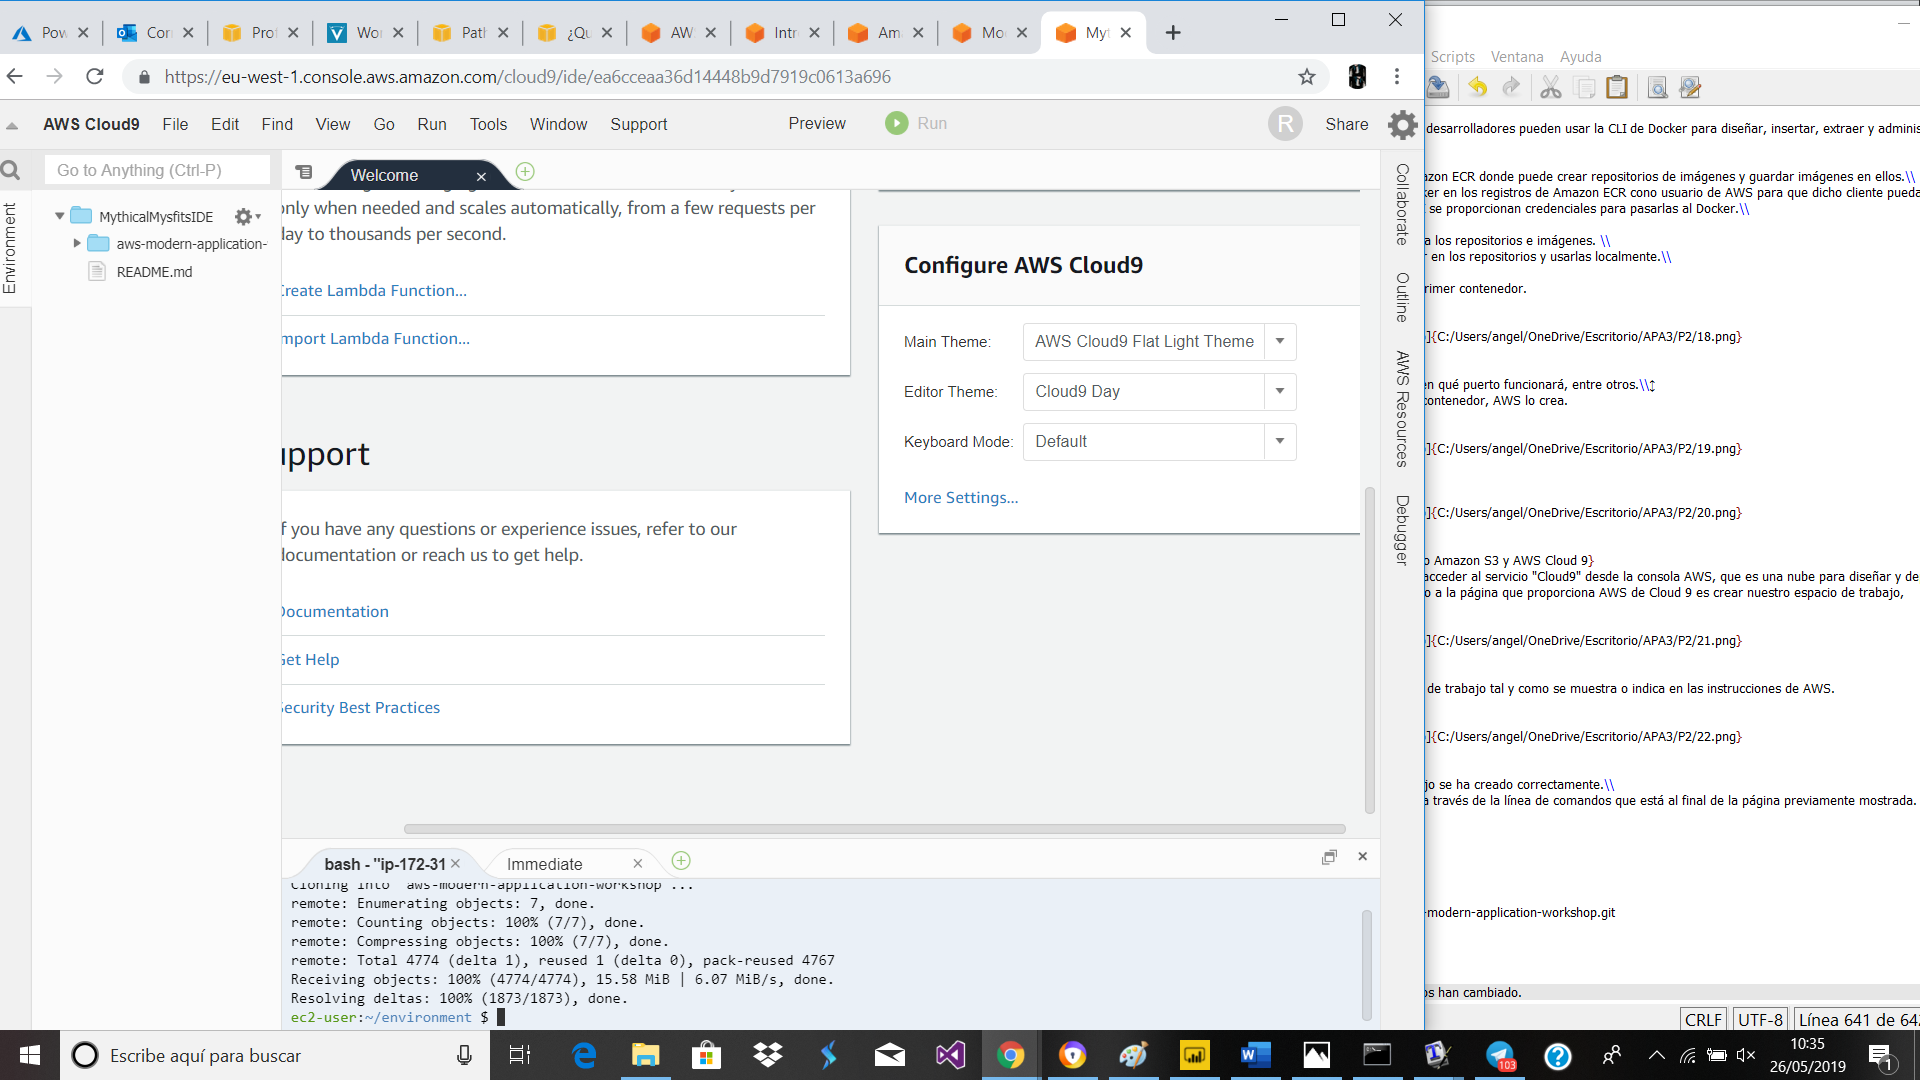
\includegraphics[width=8cm,height=8cm,keepaspectratio]{./Contenedores/AWS/23.png}
\end{nscenter}
\newline
A continuación, cambiamos de directorio.
\begin{nscenter}


\noindent\rule{10cm}{0.4pt}

cd aws-modern-application-workshop

\noindent\rule{10cm}{0.4pt}
\end{nscenter}

Siguiendo con este proceso, ahora toca creat la infaestructura donde se va a subir la página web que estamos creando.\\
Primero se va a crear un S3 bucket, y para ello hay que darle un nombre, siendo angelamoreno el nombre del bucket que yo he creado.\\
\begin{nscenter}


\noindent\rule{10cm}{0.4pt}

aws s3 mb s3://angelamoreno

\noindent\rule{10cm}{0.4pt}
\end{nscenter}
\newline
Ahora, una vez el bucket tenga nombre, vamos a configurarlo.
\begin{nscenter}


\noindent\rule{10cm}{0.4pt}

aws s3 website s3://angelamoreno --index-document index.html

\noindent\rule{10cm}{0.4pt}
\end{nscenter}
Por defecto, todos los buckets creados en AWS son privados, por lo que, para que puedan ser usados en una web pública, hay que cambiar la privacidad de dicho bucket, haciendo así que todos los objetos almacenados en él sean públicos para cualquiera. Esta configuración de la privacidad está localizada en un .json, el cuál tenemos que modificar. En concreto, el archivo que hay que modificar se llama "website-bucket-policy.json", al cuál se puede acceder a través de los archivos del Cloud 9 anteriormente comentados.
\newline
\begin{nscenter}
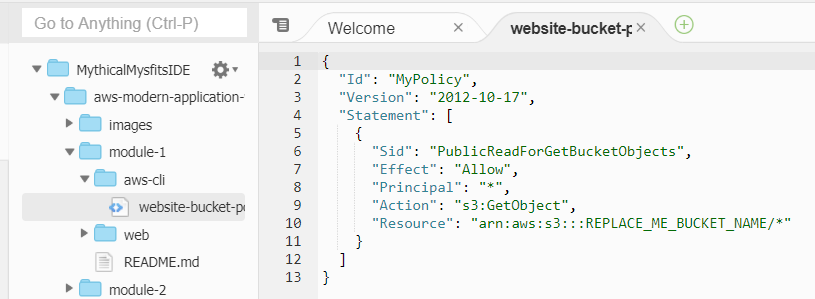
\includegraphics[width=8cm,height=8cm,keepaspectratio]{./Contenedores/AWS/24.png}
\end{nscenter}
\newline
\begin{nscenter}
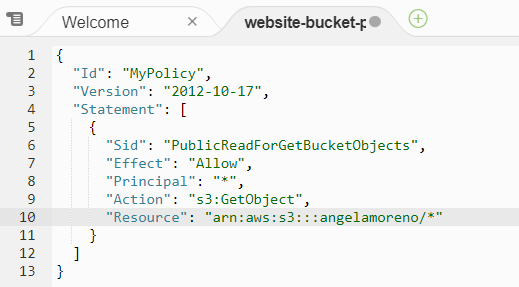
\includegraphics[width=8cm,height=8cm,keepaspectratio]{./Contenedores/AWS/25.png}
\end{nscenter}
\newline
A continuación, la siguiente instrucción se ha ejecutado a través de la CLI de AWS para terminar de configurar la privacidad del bucket.
\begin{nscenter}


\noindent\rule{10cm}{0.4pt}

aws s3api put-bucket-policy --bucket angelamoreno\\ --policy file://~/environment/aws-modern-application-workshop/module-1/aws-cli/website-bucket-policy.json

\noindent\rule{10cm}{0.4pt}
\end{nscenter}
\newline
A continuación, publicamos el contenido de la web en S3.
\begin{nscenter}
\noindent\rule{10cm}{0.4pt}
\newline
aws s3 cp\\ ~/environment/aws-modern-application-workshop/module-1/web/index.html\\ s3://angelamoreno/index.html
\noindent\rule{10cm}{0.4pt}
\end{nscenter}
\newline
Por último, una vez hecho esto, si vamos al navegador e introducimos la web que se detalla a continuación, tendremos acceso a la página web que hemos creado.
\begin{nscenter}
\noindent\rule{10cm}{0.4pt}
http://angelamoreno.s3-website-eu-west-1.amazonaws.com/
\noindent\rule{10cm}{0.4pt}
\end{nscenter}
Siendo angelamoreno el nombre del bucket y "eu-west-1" el código correspondiente de localización de Irlanda (puesto que España no aparecía como posible localización).
\newline
\begin{nscenter}
\includegraphics[width=8cm,height=8cm,keepaspectratio]{./Contenedores/AWS/26.png}
\end{nscenter}
\newline

\newpage
\subsection*{Google Cloud}
Google Cloud utiliza la aplicación 'Container Engine' (GKE) para administrar y organizar clústeres que ejecuta contenedores Docker. Container Engine programa los contenedores en el clúster y los administra automáticamente en función de los requisitos definidos (como la CPU y la memoria). Está desarrollado en el sistema Kubernetes de código abierto, lo que permite aprovechar la infraestructura de la nube pública, híbrida o in situ.

\subsubsection*{Crear un clúster con GKE}

Lo primero que hay que hacer para poder crear un clúster es crear un proyecto; esto se hace a través de la página de Kubernetes Engine.
\newline
\begin{nscenter}
\includegraphics[width=8cm,height=8cm,keepaspectratio]{./Contenedores/Googlecloud/43.png}
\end{nscenter}
\newline
A continuación hay que elegir un shell, pudiendo usar la shell local o la shell proporcionada por Google Cloud, que es la que voy a usar yo. \\
Esta shell que viene dada por Google Cloud viene peinstalada con las herramientas de línea de comandos gcloud y kubectl; proporcionando la primera la interfaz de línea de comandos principal de GCP y la segunda la interfaz de línea de comandos para ejecutar los comandos en los clústeres de Kubernetes. \\
Para configurar el proyecto creado anteriormente hay que ejecutar las siguientes instrucciones en la shell: 
\begin{nscenter}


\noindent\rule{10cm}{0.4pt}

gcloud config set project angelamorenoproyecto \\
gcloud config set compute/zone europe-west2

\noindent\rule{10cm}{0.4pt}
\end{nscenter}
\newline
Una vez que se ha configurado el proyecto, puedo proceder a crear el clúster de GKE:
\newline
\begin{nscenter}
\noindent\rule{10cm}{0.4pt}

gcloud container clusters create angelamorenocluster

\noindent\rule{10cm}{0.4pt}
\end{nscenter}
Como se puede ver en la imagen que viene a continuación, al ejecutar el comando anterior, da error. El error es debido a que Kubernetes Engine API no tenía permiso para acceder al proyecto. Haciendo click sobre la URL que se muestra en la imagen que viene a continuación pude habilitarlo.
\newline
\begin{nscenter}
\includegraphics[width=12cm,height=12cm,keepaspectratio]{./Contenedores/Googlecloud/44.png}
\end{nscenter}
\newline
Al ejecutar de nuevo la intrucción para crear el clúster volvió a dar error. Sin embargo, en esta ocasión, el error se debía a que la zona o localización elegida para el proyecto (europe-west2) no tenía la cuota necesaria como para permitir crear el clúster. Por tanto, cambié la localización del proyecto y, al volver a ejecutar la instyrucción no hubo ningún error.
\newline
\begin{nscenter}
\includegraphics[width=10cm,height=10cm,keepaspectratio]{./Contenedores/Googlecloud/45.png}
\includegraphics[width=10cm,height=10cm,keepaspectratio]{./Contenedores/Googlecloud/46.png}
\end{nscenter}
\newline
A continuación, para autenticarme y poder interactuar con el clúster ya creado, ejecuté el siguiente comando:
\begin{nscenter}


\noindent\rule{10cm}{0.4pt}

gcloud container clusters get-credentials angelamorenocluster

\noindent\rule{10cm}{0.4pt}
\end{nscenter}
Una vez que se ha creado el clúster se pueden implementar aplicaciones en contenedores en él. En esta ocasión voy a implementar una aplicación dada por Google Cloud llamada hello-app.
\subsubsection*{Implementar una aplicación en el clúster}
Para ejecutar la aplicación hello-app en el clúster que hemos creado, ejecuto el siguiente comando:
\begin{nscenter}


\noindent\rule{10cm}{0.4pt}

kubectl run hello-server --image gcr.io/google-samples/hello-app:1.0 --port 8080

\noindent\rule{10cm}{0.4pt}
\end{nscenter}
Dicho comando, al ejecutarse, va a retornar un 'hello-server created'. \\
A continuación, para exponerlo en Internet y que los usuarios puedan acceder a ella, se ejecuta el siguiente comando:
\begin{nscenter}


\noindent\rule{10cm}{0.4pt}

kubectl expose deployment hello-server --type LoadBalancer \ \\
  --port 80 --target-port 8080

\noindent\rule{10cm}{0.4pt}
\end{nscenter}

\subsubsection*{Inspeccionar y visualizar la aplicación}
Para inspeccionar el servicio hello-server y que así nos de la dirección IP externa del servicio hay que ejecutar el siguiente comando:
\begin{nscenter}


\noindent\rule{10cm}{0.4pt}

kubectl get service hello-server

\noindent\rule{10cm}{0.4pt}
\end{nscenter}
\newline
\begin{nscenter}
\includegraphics[width=8cm,height=8cm,keepaspectratio]{./Contenedores/Googlecloud/47.png}
\end{nscenter}
\newline
Si copiamos la dirección IP externa en el navegador, nos aparecerá la aplicación.
\newline
\begin{nscenter}
\includegraphics[width=8cm,height=8cm,keepaspectratio]{./Contenedores/Googlecloud/48.png}
\end{nscenter}
\subsubsection*{Limpieza}
Para borrar tanto el servicio de la aplicación como el clúster creados hay que ejecutar los siguientes comandos:
\newline
\begin{nscenter}
\includegraphics[width=8cm,height=8cm,keepaspectratio]{./Contenedores/Googlecloud/49.png}
\end{nscenter}
\newpage
\subsection*{Conclusiones}
\subsubsection*{Azure}
Con respecto a contenedores, Azure tiene cinco aplicaciones para poner trabajar con ellos. \\
1. Kubernetes Service o AKS: Es un servicio ofrecido por Azure que simplifica la implementación de clústeres. Como característica destacada encontramos que al implementar un clúster de AKS, el maestro y todos los nodos de Kubernetes se implementan y configuran automáticamente. \\
Pero, además de eso, AKS ofrece administración de identidades y seguridad a través de RBAC, que implementan las definiciones de 'rol' a un usuario o gupo para un ámbito determinado; también ofrece supervisión y registro integrados. \\
AKS también ofrece escalado de pods y nodos de clúster: a medida que cambia la demanda de recursos, el número de pods o nodos de clúster que ejecutan sus servicios pueden escalarse vertical u horizontalmente;  actualizaciones de nodos de clúster y nodos habilitados para GPU. \\
También es compatible con imágenes de Docker.\\
2. Service Fabric: Es una plataforma de sistemas distribuidos para implementar y administrar microservicios y contenedores escalables. \\
3. Azure Web App for Containers: Proporciona pilas de aplicaciones predefinidas en Linux con compatibilidad con lenguajes como .NET, PHP y Node.js entre otros. También puede usar una imagen personalizada de Docker para ejecutar la aplicación web. \\
4. Azure Container Registry: Servicio de registro de contenedores de Docker usado para almacenar imágenes de contenedor de docker privadas. \\
5. Azure Container Instances: Ejecutar contenedores de Docker sin servidor en Azure.

\subsubsection*{AWS}
Con respecto a contenedores, AWS tiene cinco servicios para trabajar con ellos: \\
1. Amazon ECR: Servicio de organización de contenedores para almacenar sus imágenes de contenedores. Facilita las tareas de almacenamiento, administración e implementación. \\
2. Amazon ECS: Dividir aplicaciones monolíticas en microservicios, migrar a la nube o ejecutar cargas de trabajo de procesamiento por lotes. Tambien aplicaciones de aprendizaje automático. \\
3. Amazon EKS: Ejecutar Kubernetes en AWS, crear aplicaciones híbridas o implementar modelos de aprendizaje automático. \\
4. AWS Fargate: Contenedores sin servidor o crear una PaaS. \\
5. Amazon EC2: Obtener el máximo control sobre su tipo de lanzamiento.

\subsubsection*{Google Cloud}
Google Cloud tiene Container Engine como sistema de administración y organización de clústeres que ejecuta contenedores Docker. \\
Container Engine es compatible con Docker, tiene registro privado de contenedores para almacenar imágenes Docker privadas y acceder a ellas fácilmente, es escalable, tiene logging y monitoring, permite redes híbridas y administración de identidades y acceso.
\newline
Como conclusión, de Azure destacaría la gran cantidad de tutoriales que tienen disponibles, pudiendo haber creado un clúster, una aplicación en un contenedor, crear una aplicación web, crear un grupo de recursos, crear un registro de Docker privado y añadirle una imagen. \\ 
De AWS destacaría lo intuitivo que es, además de un punto muy importante en temas de seguridad que es la generación de las dos claves, además de la generación de un ID y contraseña secretos cuando intentas acceder de forma remota. También destaco la cantidad de tutoriales y de ejemplos que hay en la web, la documentación, además del procesamiento en lotes y las aplicaciones de aprendizaje automático. Además, también destacaría AWS Cloud9, que permite escribir, ejecutar y debuggear código en el propio buscador. Como punto negativo, pondría que para poder acceder a tutoriales no sirve con la cuenta AWS student. \\
Con respecto a Google Cloud, destaco el tener una única aplicación para trabajar con los contenedores, además de permitir redes híbridas, logging y monitoring. Sin embargo, ampliaría la documentación que ofrecen, al igual que tutoriales. 
\newline
Por todo lo anteriormente comentado e implementado, mi elección sería AWS.

\newpage
\subsection*{Problemas encontrados}
Durante el desarrollo de esta práctica he encontrado mayoritariamente un problema, y es que me ha sido imposible instalar Docker en el ordenador Windows que tengo, debido a que, como se ha comentado anteriormente, Docker pide tener como sistema operativo Windows 10 Pro, el cual yo no tengo. \\
Por tanto, para solucionar ese problema, hay apartados de la práctica que han sido resueltos con el sistema operativo Windows y otros (cuando daba algún tipo de error en Windows) con el sistema operativo macOS Sierra.
\newline
\begin{nscenter}
\includegraphics[width=10cm,height=10cm,keepaspectratio]{./Contenedores/Googlecloud/50.png}
\end{nscenter}
\newpage
\subsection*{Bibliografía containers}

1. Shell de Azure: https://shell.azure.com/ \\
2. Azure for Containers: https://docs.microsoft.com/es-es/azure/containers/ \\
3. Instalación de la CLI de Azure en macOS: https://docs.microsoft.com/es-es/cli/azure/install-azure-cli-macos?view=azure-cli-latest \\
4. Introducción a los contenedores (AWS): https://aws.amazon.com/es/containers/getting-started/ \\
5. Container Engine - Google Cloud: https://cloud.google.com/container-engine/?hl=es
\end{document}